\documentclass[pdftex,english,10pt,b5paper,twoside]{book}
\usepackage[T1]{fontenc} % In case we want special characters
\usepackage[utf8]{inputenc} % We are all writing in UTF-8

\usepackage[numbers]{natbib} % We need to tweak our referencing a bit.
\usepackage{appendix} % Fixes formatting of appendices
\usepackage[printonlyused]{acronym} % Package to handle the acronym list
\usepackage{graphicx} % We *may* use images
\graphicspath{{images/}} % and it is clean to put them in a separate dir
\usepackage{hyperref} % Internal and external links is nice
\hypersetup{pdfborder=0 0 0} % ..especially without red borders
\usepackage{amstext} % To support \text in math mode

% Packages and settings for code listings
\usepackage{listings}
\usepackage{caption}
\usepackage{upquote}
\usepackage{xcolor}
\DeclareCaptionFont{white}{\color{white}}
\DeclareCaptionFormat{listing}{\colorbox{gray}{\parbox{\textwidth}{#1#2#3}}}
\captionsetup[lstlisting]{format=listing,labelfont=white,textfont=white}
\lstset{
language=Java,
keywordstyle=\bfseries\ttfamily\color[rgb]{0,0,1},
identifierstyle=\ttfamily,
commentstyle=\color[rgb]{0.133,0.545,0.133},
stringstyle=\ttfamily\color[rgb]{0.627,0.126,0.941},
showstringspaces=false,
basicstyle=\small,
numberstyle=\footnotesize,
numbers=left,
stepnumber=1,
numbersep=10pt,
tabsize=2,
breaklines=true,
prebreak = \raisebox{0ex}[0ex][0ex]{\ensuremath{\hookleftarrow}},
breakatwhitespace=false,
aboveskip={1.5\baselineskip},
columns=fixed,
upquote=true,
extendedchars=true,
frame=bottomline,
inputencoding=utf8
}

% Set equal margins on book style
% \usepackage{layout} % Use \layout to print out the margins (debug)
%\usepackage{geometry}
%\geometry{bindingoffset=1cm}
\usepackage[lmargin=25mm,rmargin=25mm,tmargin=27mm,bmargin=30mm]{geometry}

% Restyle chapter headers
\usepackage{fix-cm}
\makeatletter
\renewcommand{\@makechapterhead}[1]{%
  \vspace*{50\p@}%
  {\parindent \z@ \raggedright \normalfont
    \vspace{15pt}%
    \ifnum \c@secnumdepth >\m@ne
        %\hfill\huge\scshape \@chapapp\space
        \hfill\fontsize{60}{90}\selectfont \thechapter % Chapter number
        \par\nobreak
        \vskip 20\p@
    \fi
    \interlinepenalty\@M
    \hfill \Huge \scshape #1\par % Chapter title
    \vspace{5pt}
    \hrule
    \nobreak
    \vskip 40\p@
  }}
\makeatother

\author{Eirik Haver \and Eivind Melvold \and Pål Ruud}
\title{Master thesis - Cloud Storage Vault}
\date{\today}

\begin{document}

\include{title}
\pagestyle{empty}

\chapter*{Abstract}
\addcontentsline{toc}{chapter}{Abstract}
\pagestyle{plain}
\pagenumbering{Roman}
\setcounter{page}{1}

%  Writers should follow a checklist consisting of:
% Motivation: Why do we care about the problem and results?
% Problem Statement: What problem are we trying to solve? Scope/limits.
% Approach: How did we go about solving or making progress on the problem?
% Results: What is the answer? Numbers, not vague 'very', 'small' etc.
% Conclusions: What are the implications of your answer? Further work.
%
%  Each section is typically a single sentence, although there is room for
%  creativity.

\chapter*{Preface}
\addcontentsline{toc}{chapter}{Preface}

The work behind this project report was carried out during the spring semester
in 2011 at the Norwegian University of Science and Technology (NTNU), Department
of Telematics (ITEM).
\vspace{13pt}

\begin{center}
Eirik Haver, Eivind Melvold and Pål Ruud
\vspace{13pt}

\end{center}

\tableofcontents

\cleardoublepage
\phantomsection
\addcontentsline{toc}{chapter}{\listfigurename}
\listoffigures

\cleardoublepage
\phantomsection
\addcontentsline{toc}{chapter}{\listtablename}
\listoftables

\cleardoublepage
\phantomsection
\addcontentsline{toc}{chapter}{\lstlistlistingname}
\lstlistoflistings
\cleardoublepage

\chapter*{Acronyms}
\addcontentsline{toc}{chapter}{Acronyms}

\begin{acronym}
\acro{ACL}{Access Control List}
\acro{AES}{Advanced Encryption Standard}
\acro{API}{Application Programming Interface}
\acro{BC}{Bouncy Castle}
\acro{CA}{Certification Authority}
\acro{CBC}{Cipher Block Chaining}
\acro{CDA}{Cluster Dictionary Attack}
\acro{CG}{Credential Generator}
\acro{CM}{Cloud Manager}
\acro{CPU}{Central Processing Unit}
\acro{DP}{Data Processor}
\acro{DRY}{Don't Repeat Yourself}
\acro{DSA}{Digital Signature Algorithm}
\acro{DSS}{Digital Signature Scheme}
\acro{DV}{Data Verifier}
\acro{EC2}{Elastic Compute Cloud}
\acro{ECB}{Electronic Codeboo}
\acro{ETE}{External Trusted Entity}
\acro{FAQ}{Frequently Asked Questions}
\acro{HDFS}{Hadoop Distributed File System}
\acro{HTTP}{Hypertext Transfer Protocol}
\acro{HTTPS}{Hypertext Transfer Protocol Secure}
\acro{IaaS}{Infrastructure as a Service}
\acro{IV}{Initialization Vector}
\acro{JCA}{Java Cryptography Architecture}
\acro{JCE}{Java Cryptographic Extensions}
\acro{JDK}{Java Development Kit}
\acro{JRE}{Java Runtime Environment}
\acro{JVM}{Java Virtual Machine}
\acro{LAFS}{Least Authority File System}
\acro{MITM}{Man-in-the-middle}
\acro{NIST}{National Institute of Standards and Technology}
\acro{PBKDF2}{Password-Based Key Derivation Function version 2}
\acro{PaaS}{Platform as a Service}
\acro{PasS}{Privacy as a Service}
\acro{PEP}{Python Enhancement Proposal}
\acro{PGP}{Pretty Good Privacy}
\acro{PKI}{Public Key Infrastructure}
\acro{PoC}{Proof-of-concept}
\acro{QR}{Quick Response}
\acro{RAM}{Random access memory}
\acro{REST}{Representational State Transfer}
\acro{RSA}{Rivest, Shamir and Adleman}
\acro{SaaS}{Software as a Service}
\acro{SDK}{Software Development Kit}
\acro{SHA}{Secure Hash Algorithm}
\acro{SQL}{Structured Query Language}
\acro{SSL}{Secure Socket Layer}
\acro{TC}{Trusted Coordinator}
\acro{TCCP}{Trusted Cloud Computing Platform}
\acro{TCG}{Trusted Computing Group}
\acro{TG}{Token Generator}
\acro{TLS}{Transport Layer Security}
\acro{TPM}{Trusted Platform Module}
\acro{TTP}{Trusted Third Party}
\acro{TVMM}{Trusted Virtual Machine Monitor}
\acro{URI}{Uniform Resource Indetifier}
\acro{URL}{Uniform Resource Locator}
\acro{VM}{Virtual Machine}
\acro{VMM}{Virtual Machine Monitor}
\acro{WSGI}{Web Server Gateway Interface}
\end{acronym}

%**************************************%
\chapter{Introduction}
%**************************************%
\pagenumbering{arabic}
\setcounter{page}{1}

\section{Method}

\section{Outline}

The work is presented as per the following chapters:

\paragraph{Chapter 2} provides background knowledge of the technologies and
software used.


%**************************************%
\chapter{Background}
%**************************************%

\section{Security Services}

This section explains certain security services used in this thesis. A security
service is any processing or communication service that enhances the security of
the data processing systems and the information transfers of any organization
\cite[p. 12]{stallings}.

\paragraph{Confidentiality} Confidentiality is the act of keeping a message
secret from unauthorized parties \cite[p. 18]{stallings}. This can typically be
done by either preventing other parties access to the message at all, or making
the contents unreadable, for instance by the use of encryption.

\paragraph{Integrity} Integrity in a security perspective deals with detecting,
preventing or recovering a message being changed by an unauthorized party
\cite{stallings}.

\paragraph{Authentication} Authentication is the act for a user, service or
similar to prove that he is what he claims to be \cite{stallings}.

\paragraph{Nonrepudiation} Nonrepudiation prevents both sender and receiver of
a message from denying a transmitted message, in other words one party can
prove the other parties involvement \cite{stallings}.

\section{Cryptographic Primitives}

This section explains the low level security primitives used in this thesis.

\subsection{Encryption}

Encryption is the process of transforming some information into an unreadable
form. Encryption is primarily used to enforce Confidentially, but can also be
used for other purposes such as authentication.  In a very basic form an
encryption scheme consist of an encryption algorithm, the \emph{cipher}, a key
and a message, the \emph{plaintext}, that is all used to create an encrypted
message, the \emph{ciphertext}. If a good cipher is used, knowledge of the
cipher, multiple plaintext and multiple ciphertext should not be enough to
obtain the key or decrypt ciphertext with a corresponding unknown
plaintext\cite[p. 30]{stallings}.

\paragraph{Block-cipher and Stream-cipher} are classifications on how a cipher
treats data\cite[p. 32]{stallings}. A block cipher will encrypt a block of data
of a specific size. If the data is larger than the block size used by the
application a \emph{mode of operation} is needed. In a stream cipher the
plaintext will usually be combined with a pseudorandom key stream to generate
the plaintext.

\paragraph{Symmetric encryption} is an encryption scheme where the same key is
used for both encryption and decryption\cite[p. 32]{stallings}. \ac{AES} is a
block cipher and is the current standard for symmetric encryption. \ac{AES}
works on a block of 128-bit and support keys of 128, 192 and 256-bit.

\paragraph{The mode of operation} used for a symmetric encryption enables
subsequent safe use of the same key. In a simple scenario this could be to
encrypt the normal data block-by-block with pure \ac{AES}, which is called the
\ac{ECB} mode of operation. The problem with this is that some information of
the ciphertext will leak, i.e. the same plaintext will always be the same
ciphertext. A more usefull way is \emph{\ac{CBC}}. In \ac{CBC} you will need an
\ac{IV} which should be non-predictable, and not reused. The \ac{IV} is XORed
with the first block of plaintext, which again is encrypted with \ac{AES}. The
resulting ciphertext is used as an \ac{IV} for the next block\cite[p. 183]{stallings}.

\paragraph{Asymmetric encryption} is an encryption scheme where a different key
is used for encryption than decryption\cite[p. 259]{stallings}. An asymmetric
encryption scheme is often called a public-key encryption scheme, where one key
is defined as private and the other as public. The public key is shared to
allow other parties to encrypt messages for the owner of the private key. The
downside of asymmetric encryption compared to symmetric is that it requires a
larger key and has a larger computational overhead to obtain the same level of
confidentiality. The probably best known asymmetric cipher is \ac{RSA}.

\subsection{Cryptographic hash functions}
A cryptographic hash function is a deterministic mathematical procedure which
takes an arbitrary block of data and outputs a fixed-size bit string. The output
is referred to as the hash value, message digest or simply digest.
Another property of a cryptographic hash function is that the smallest change in
the input data (e.g. one bit) should completely change the output of the hash
function. In other words it should be infeasible to find the reverse of a
cryptographic hash function \cite[p. 335]{stallings}. It should also be infeasible to
find two blocks of data which produce the same hash value (a \emph{collision}).

The standard for cryptographic hash functions today are \ac{SHA}-1 and the
\ac{SHA}-2 family.

\section{Applications of cryptographic primitives}

\subsection{Digital Signatures}
A digital signature is the digital equivalent of a normal signature, it
verifies that an entity approves with or has written a message, the date the
signature was made and it should be verifiable by a third party \cite[p.
379]{stallings}. It should logically not be possible or at least unfeasible to
fake a digital signature. It is possible to create digital signatures with
\ac{RSA} there is also a standard for digital signatures called \ac{DSS} which
uses \ac{DSA} as the actual algorithm.

\subsection{Digital Certificates and PKI} A digital certificate is the pairing
of a digital signature and a public key\cite{stallings}.  By this scheme the
services confidentiality, authentication and nonrepudiation can be achieved.
Basically a person or other entity has a certificate with some clues about the
identity in it, e.g. the e-mail, together with a public key. This certificate
can then be signed using digital signatures to verify that some other entity
trusts this certificate. In practise the entity which signs certificates is the
\ac{CA} which all clients have the public key information for, and trusts. The
\ac{CA} will also contain information about which certificates has been
revoked, i.e. should not be trusted in use. Such a scheme is usually referred
to as a \ac{PKI}.

\subsubsection{PGP} \ac{PGP} is a scheme similar to \ac{PKI} but with no
\ac{CA} that all users trusts\cite{stallings}. Instead trust is made between
users by somehow verifying their public key, for instance by meeting face to
face. A user can then sign another users key, set a trust level for the user
and publish this information to a keyserver. Another user can then calculate a
trust to an unknown person based on the trust set by peoples that he trusts.

\subsection{SSL/TLS}
\ac{TLS} and its predecessor \ac{SSL} are techniques for obtaining
confidentiality, integrity for transfer of files over a
network\cite{stallings}. It does so by a combination of different algorithms
and primitives, but a digital certificate is required for authentication.

\subsection{PBKDF2}
\label{sec:PBKDF2}
\ac{PBKDF2} is a key derivation function to create an encryption key based on
a password. The point of this is that a password is often something that should
be memorable to a person, but what is memorable to a person might be a to short
phrase to withstand a brute force attack. What \ac{PBKDF2} does is make the
process of deriving the key from the password an expensive process in terms of
computational power, to make it more resistant to brute force attacks. A feature
known as key stretching. The efficiency of the key derivation is dependent on the
number of process iterations chosen for the function.

\section{Security Attacks}
This section briefly list security attacks relevant to this thesis, as defined
by \citeauthor{stallings}.
%TODO: Mulig man skal bruke en annen måte å refere kilden på her

\paragraph{Active and passive attacks} are classifications of security attacks,
where a passive attack attempts to learn or make use of information from the
system but does not affect system resources. An active attack attempts to alter
system resources or affect their operation.

\paragraph{Traffic analysis} Traffic Analysis is the act of capturing
communication sent between two parties. This information might contain secrets
or might for instance leak enough information about an encryption key to make
it breakable.

\paragraph{Masquerade} Masquerade is an active attack where the attacker pretends to be
one of the legit parties.

\paragraph{Replay} Replay is an active attack where the attacker capture some data in
a communication session and subsequently retransmit that information.

\paragraph{Modification of messages} Modification of messages is an active attack where the attacker
alters some of the contents of a message sent between two communicating
parties.

\paragraph{Denial of Service} Denial of Service is an active attack where the attacker seeks to
make resources unavailable for legit users, i.e. by overloading an application
by sending it lots of traffic.

\paragraph{\acl{MITM}} \ac{MITM} is an attack where an attacker intercepts messages
between the communicating parties and then either relay or substitute the
intercepted message.

\subsection{Attacks on cryptographic primitives}
Even though cryptographic primitives are designed to be secure, they might have
both flaws and be used in an incorrect fashion.

\paragraph{Cryptanalysis attack} is an attempt to deduce a specific plaintext
or to deduce the key being used in a ciphertext.

\paragraph{Brute-force attack} In a brute-force attack an attacker tries
to obtain a secret by testing the algorithm with up to all possible inputs. The
secret might be an encryption key or the data fed into a cryptographic hash
function. A related attack is the \emph{Dictionary attack} where the attacker
tries to obtain a secret by trying a subset of all known inputs, the ones
defines in his dictionary.  

\section{Cloud Computing}
In a draft\cite{cloud_nistdef} \ac{NIST} defines cloud computing as:
\begin{quote}
Cloud computing is a model for enabling ubiquitous, convenient,
on-demand network access to a shared pool of configurable computing resources
(e.g., networks, servers, storage, applications, and services) that can be
rapidly provisioned and released with minimal management effort or service
provider interaction.
\end{quote}

\subsection{Service Models}
\ac{NIST} also defines three service models which deals with what kind of
service the consumer is able to rent from a provider.

\paragraph{\ac{SaaS}} is the capability for a consumer to run the provider's
application running on cloud infrastructure, using a thin-client, browser or
similar. Gmail\footnote{\url{http://www.gmail.com}} can be seen as an example
of this.

\paragraph{\ac{PaaS}} is the capability for a consumer to deploy software onto
the cloud, but without actually controlling the underlying platform, operating
system etc.

\paragraph{\ac{IaaS}} is the capability provided to the consumer to provision
processing, storage, networks and other fundamental computing resources where
he can run arbitrary software, including operating systems and applications. An
example is hiring a \ac{VM}.

\subsection{Deployment Models}
The \ac{NIST} draft also lists several Deployment Models which deals with how
the cloud is organized in terms of where it is hosted and who has access to it.

\paragraph{Private Cloud} is a cloud infrastructure operated solely for an
organization. Which party manages the cloud and where it is located is not
given.

\paragraph{Community Cloud} is a cloud infrastructure is shared by several
organizations to serve a common concern. Where it is located and who manages it
is not given.

\paragraph{Public Cloud} is a cloud infrastructure where basically everyone or
at least a large group can have access, and is owned by a external provider of
cloud services.

\paragraph{Hybrid Cloud} is a cloud infrastructure composed of two or more
clouds of any other model.

\subsection{Security considerations}
There are some considerations when using cloud services from an external provider
as opposed to self controlled hardware, software and plattforms. Most notably
is that you loose the control of selecting the people which will have physical
and digital access to the infrastructure. In essence this means that the
provider can read every data sent to and from the cloud as well as the data
saved in the cloud.

Another risk is that information might be leaked to other users of the same
cloud. For instance it might be able possible for a \ac{VM} to leak information
to other \ac{VM}s on the same host.
%TODO: kilde

%**************************************%
\chapter{Related Work}
%**************************************%

\section{Research}
This section will elaborate on previous research concerning privacy within cloud
computing. Previous research can be divided into proactive solutions that
either reduce or prevent the risk of leaking privacy related information. The
latter type of solutions are discussed.

\subsection{Privacy as a Service}
A concept entitled \ac{PasS} was suggested in 2009
\cite{PasS}. PasS is a set of security protocols ensuring privacy of customer
data in cloud computing architectures. The main design goal with PasS is to
maximize the user's control over his/her sensitive data both processed and stored
within a cloud.

To be operational, PasS is dependent on a fundamental system and trust model. The
system model consists of 3 communicating parties, namely a cloud provider, a
cloud customer and a \ac{TTP}. The PasS system model is shown
in Figure \ref{fig:RW:PasS}. 
\begin{figure}[h!]
    \centering
    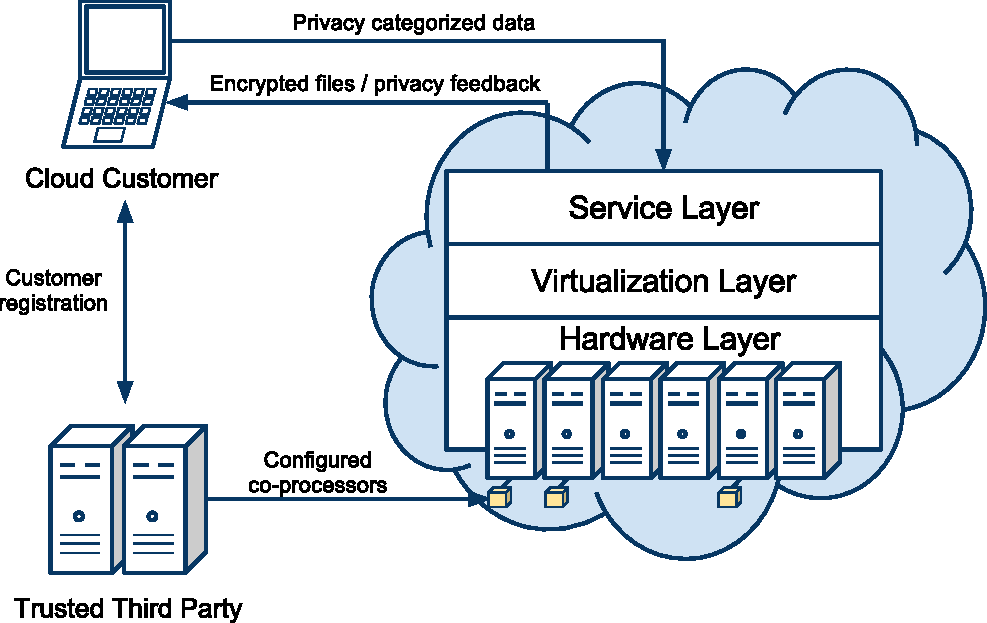
\includegraphics[scale=0.6]{ArchitecturePasS.pdf}
    \caption{System model of PasS}
    \label{fig:RW:PasS}
\end{figure}
It is important to notice that the PasS system model is dependent on
pre-installed cryptographic coprocessors in the cloud. A cryptographic
coprocessor is a small hardware card, including a processor, RAM, ROM, backup
battery, persistent storage and an Ethernet network card. A coprocessor interfaces
with a server in the cloud and provides a safe environment for processing of
a customer's sensitive/private data. The cryptographic coprocessors are used in the
cloud because they are tamper-proof against physical attacks. The coprocessors
are pre-configured by the TTP before they are installed in the cloud. In this
way, the TTP provides a safe computational environment for the cloud customer,
which is kept secret from the cloud provider.

The main task of the TTP is to compute a set of public/private key pairs, load
them into the co-processor's persistent storage in the cloud, and
further send them to the customer. The TTP also loads its own secret key into
the coprocessor. This key distribution ensures secure communication between the
TTP, coprocessors and the cloud customer. The customer's key pair is sent through a
secure communication channel.

With cryptographic coprocessors in the cloud and a secure communication, the
cloud customer can choose between 3 different levels of privacy towards the
cloud provider. The customer can choose between no privacy, privacy with trusted
provider and privacy with none-trusted provider.

No privacy equals storing data as clear text in the cloud. Privacy with trusted
provider involves storing encrypted data in the cloud. This data is encrypted by
the cloud provider and only achievable by the customer or cloud provider.
In the case of privacy with non-trusted provider, the customer encrypts the
private data before uploading it to the cloud provider. The key used for
encryption is shared with the cryptographic co-processor, through an
authenticated version of the Diffie-Hellman key management protocol. The
co-processor can further process the encrypted data and store it in the cloud
facility. The stored data is encrypted and unknown to the cloud provider.

\subsection{Privacy Manager}
In 2009, HP Labs proposed a way to manage and control a user's private data stored and
processed in a cloud facility \cite{privacymanager}. Their solution was partially implemented
as a software program called a privacy manager.

The privacy manager uses a feature/method called obfuscation, which is quite similar to
encryption. However, the obfuscation method is different from encryption, in the
sense that the obfuscated data can be processed in the cloud, without the cloud
provider knowing the encryption key or the original data. \cite{privacymanager} mention the following
obfuscation methods:
\begin{itemize}
\item Yao's protocol for secure two-party computation \cite{yao}
\item Gentry's homomorphic encryption scheme \cite{gentry}
\item Narayanan and Schmatikov's obfuscation method \cite{obfuscationmethod}
\end{itemize}
Due to better efficiency, the privacy manager uses the latter alternative. However,
Narayanan and Schmatikov's obfuscation method does not provide complete
confidentiality to the cloud provider \cite{obfuscationmethod}.

In addition to installing a privacy manager at the user's terminal, HP Labs suggests
the use of trusted computing solutions to address the lower-level protection of
data. The \ac{TCG} is an example of an organization
developing and providing trusted computing solutions \cite{tcg}. HP Labs
suggests using a tamper-proof piece of hardware called a \ac{TPM}, which is
designed by TCG. The TPM is installed in the machine running the
privacy manager to ensure that processes carried out by the privacy manager can be
fully trusted.

The privacy manager is suggested to work in 3 different use cases. It can be
implemented to support a single client, the use of hybrid clouds and/or the use of an
infomediary within the cloud.

%Regarding applications in the cloud where users have to upload unobfuscated
%private data, the privacy manager includes two additional features called
%preferences and personae. Both features are dependent on a trustworthy service
%and cloud provider, and are therefore irrelevant to our development.

\subsection{Trusted Cloud Computing Platform}
Equal to PasS and the privacy manager, \ac{TCCP} was proposed as a solution to
provide secure computations (and storage) within a non-trusted cloud provider
\cite{tccp}. As opposed to the previous solutions, TCCP is directed against secure
execution of guest VMs outsourced to IaaS providers. 

The original IaaS structure, before adding TCCP, is assumed to consist of a
\ac{CM}, which manages a cluster of nodes running one or more VMs. Among
multiple tasks, the CM is responsible for loading VM images into its own nodes.
Each node has a \ac{VMM} which will further launch and monitor VMs from the
received VM images.

TCCP is based upon the fundamental TPM chip designed by the TCG. The TPM
contains a private/public key pair that uniquely identifies the TPM. The public
key is additionally signed by the manufacturer to guarantee correctness of
the TPM chip. With this in mind, TCCP is based upon a remote attestation scheme.
The remote attestation scheme enables a network entity to verify whether another
remote entity runs a TPM or not. A detailed description of the remote
attestation scheme is given in \cite{tccp}.
\begin{figure}[h!]
    \centering
    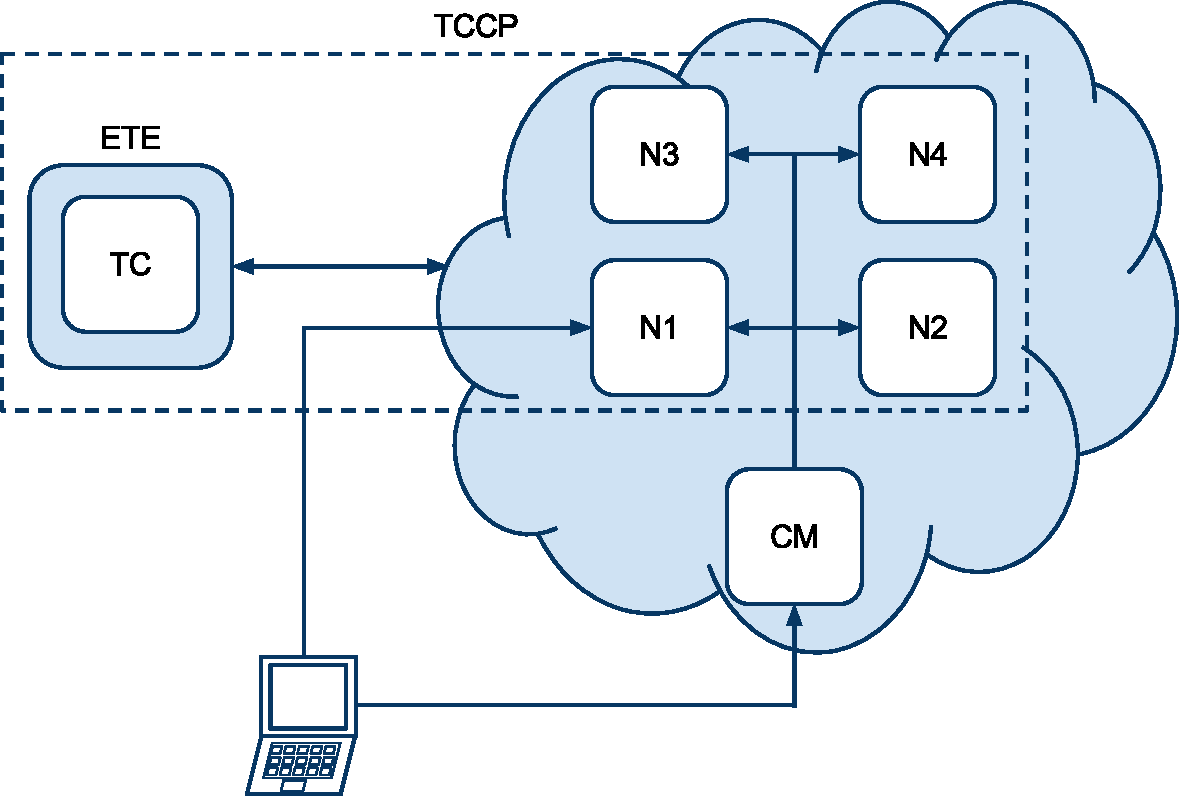
\includegraphics[scale=0.4]{ArchitectureTCCP.pdf}
    \caption{System architecture of TCCP}
    \label{fig:RW:TCCP}
\end{figure}
The TCCP system architecture is illustrated in Figure \ref{fig:RW:TCCP}. The
trusted computing base of TCCP includes a \ac{TC} and a \ac{TVMM}. The TC
manages the trusted nodes within a cluster. To be trusted, a node must be
located within a security perimeter and run a TVMM. The TC maintains a record of
the nodes located in the security perimeter and use remote attestation to ensure
nodes are trusted. Each trusted node in a cluster contains a TPM and a
corresponding TVMM. The main task of a TVMM is to enforce a local closed box
protection of a client's running VM. Details about the TVMM design are given in
\cite{tvmm}. 

Each TVMM cooperates with a TC to protect the transmission of VMs between
trusted nodes and to ensure that VMs are executed by trusted nodes. In this
context, the TCCP specifies several protocols for both launching and migrating
VMs inside the cloud. These protocols are described in \cite{tccp}.

The TC is installed in an \ac{ETE}, maintained by a trusted third party, to prevent illegal tampering
from the IaaS provider. A client can further use remote attestation to the TC to
verify that the IaaS provider secures its computation.

With TCCP the client interacts with the IaaS provider as usual. The difference
is that the trusted nodes and their TC communicates to ensure a secure environment for executing
the client's VM.

\subsection{Cryptographic Cloud Storage}
In 2010, researchers at Microsoft were looking at the problem of building a secure
cloud storage service on top of a non-trusted cloud storage provider
\cite{microsoftresearch}. They described architectural solutions related to both consumers and
enterprises. The architectures were explained in high level and were designed to
utilize and combine recent and non-standard cryptographic primitives.

The consumer architecture is depicted in Figure \ref{fig:RW:CCS:CA}. A typical
enterprise architecture is shown in Figure \ref{fig:RW:CCS:EA}.
\begin{figure}[h!]
    \centering
    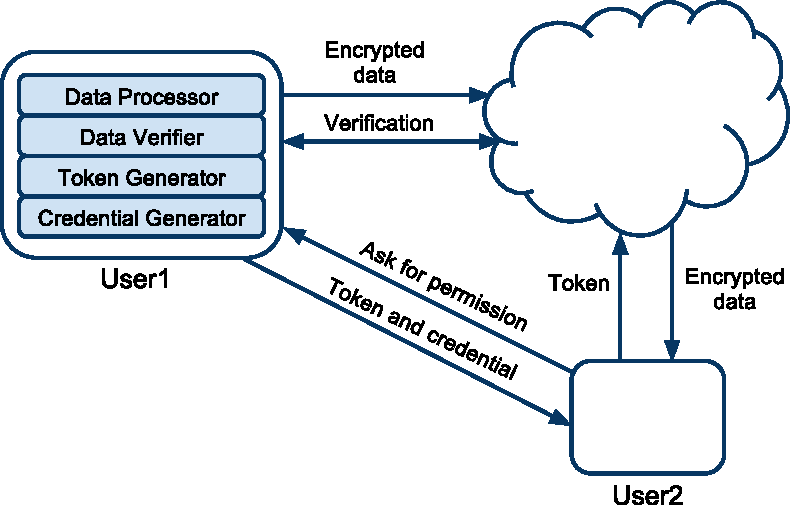
\includegraphics[scale=0.6]{ArchitectureCCSC.pdf}
    \caption{Cryptographic cloud storage, customer scenario.}
    \label{fig:RW:CCS:CA}
\end{figure}
\begin{figure}[h!]
    \centering
    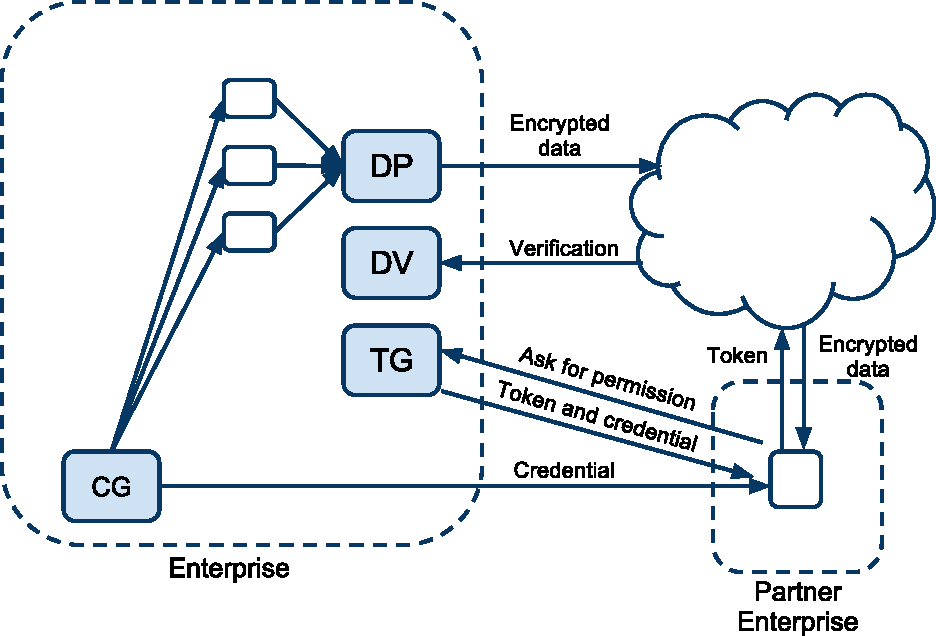
\includegraphics[scale=0.6]{ArchitectureCCSE.pdf}
    \caption{Cryptographic cloud storage, enterprise scenario.}
    \label{fig:RW:CCS:EA}
\end{figure}\\
Each architecture consists of the following computational components:
\begin{description}
\item[\ac{DP}] \hfill \\Processes data before it is sent to the cloud.
\item[\ac{DV}] \hfill \\Checks whether data stored in the cloud has been
tampered with.
\item[\ac{TG}] \hfill \\Generates tokens that enable the cloud provider to
retrieve segments of customer data.
\item[\ac{CG}] \hfill \\Responsible for creating and distributing access 
policies.
\end{description}
The core components are suggested to support searchable encryption,
attribute-based encryption and a ``proofs of storage'' protocol.

\section{Existing Solutions}
There are a number of existing solutions for storing data in the cloud,
with more or less of the functionality required to fulfill the problem
description for this thesis. The section highlights some of them.

\subsection{Dropbox}

Dropbox\footnote{\url{http://www.dropbox.com/}} is a popular commercial
application for storing data in the cloud, claiming more than 25 million users
\cite{dropbox_users}. All files are saved using Amazons S3 storage service.

The company boasts strong encryption and strict access control
\cite{dropbox_security}, but has received criticism for its lack of security
\cite{dropbox_concerns}. Among these concerns, is the \emph{Forgotten Password}
feature, which implies that Dropbox can read the users files if they really want
to, and that the encryption is performed server side.

In addition, Dropbox is not Open Source, and hence one has no way of verifying
that the security features actually work as claimed.

\subsection{Tahoe-LAFS}
% TODO: Reference cloud security software "checklist" in Intro

Tahoe-\ac{LAFS}\footnote{\url{http://www.tahoe-lafs.org/}} is an open source
secure cloud storage file system which does fulfill the requirements set by our
problem description in regards to security \cite{tahoe}. 

In Tahoe-\ac{LAFS}, files are exclusivly encrypted client-side, before beeing
uploaded into the cloud. Tahoe-\ac{LAFS} also uses erasure-coding to obtain
redundancy across multiple storage servers.

\subsection{Wuala}

Wuala\footnote{\url{http://www.wuala.com/}} is a closed source secure cloud
storage file system, that seamingly operates very similar to Tahoe-\ac{LAFS}.

The authors have released a paper on a cryptographic tree structure for file
systems, called Cryptree \cite{cryptree}, and has strong focus on reliability
by both providing central servers, in addition to a \emph{P2P cloud} of Wuala
users that has donated capacity to the system. 

%**************************************%
\chapter{Architectural Overview}
%**************************************%
\label{chap:AS}

The architectural solution of a secure cloud file sharing system has to convince
its users that the functions indeed are secure, and that the concepts are easy
to understand and accept. 

The architecture has to support various user functionality. Figure
\ref{fig:AS:overview} exhibits Alice uploading files to the cloud, and
thereafter transferring the necessary information to Bob so that he also can
gain access to the files.

In the following sections, we will describe how the file storage is organized,
and take a closer look at how the different problems are solved.

\begin{figure}[h!]
    \centering
    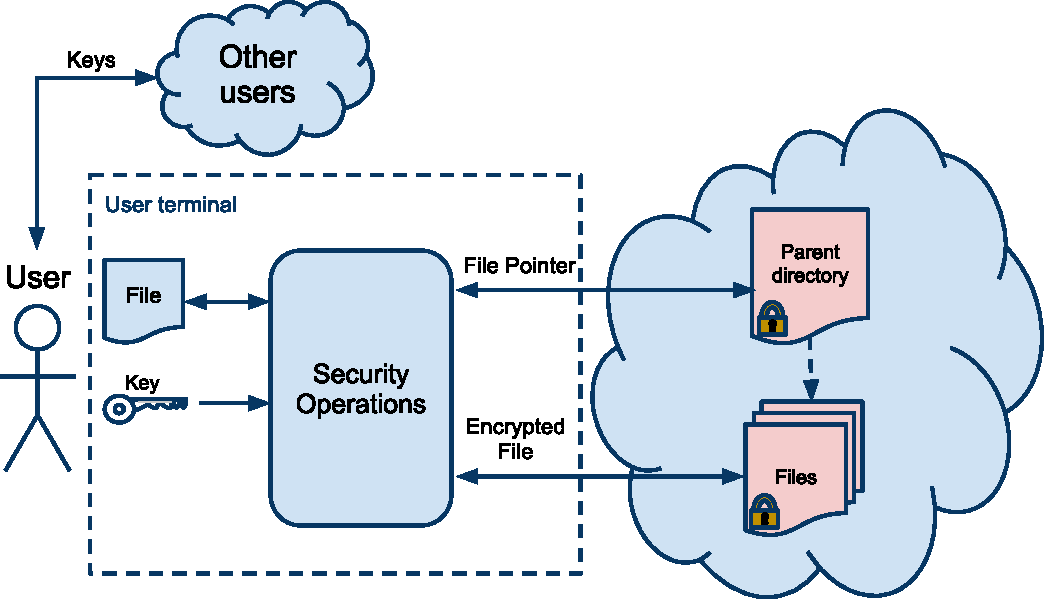
\includegraphics[width=\columnwidth]{ArchitectureOverview.pdf}
    \caption{Overview of user functionality}
    \label{fig:AS:overview}
\end{figure}

\section{File Storage}
\label{sec:AS:FS}

The solution proposed in this thesis, is that only a simple key-value store is
needed on the server side. This may be extended with an \ac{ACL} layer to
support user access and other features.

Two types of files exist: immutable and mutable files. The mutable files are used
as directories, in the sense that they contain the information needed to access
other directories or files in the form of capabilities.
A capability is a short alphanumeric string containing all information needed
to find, get, read and write a file or folder. This includes an identifier and
cryptographic keys.

In principle, the only operations the key-value store need to support, are
\textbf{PUT} and \textbf{GET}.

\subsection{Directory Structure}

\begin{figure}[h!]
    \centering
    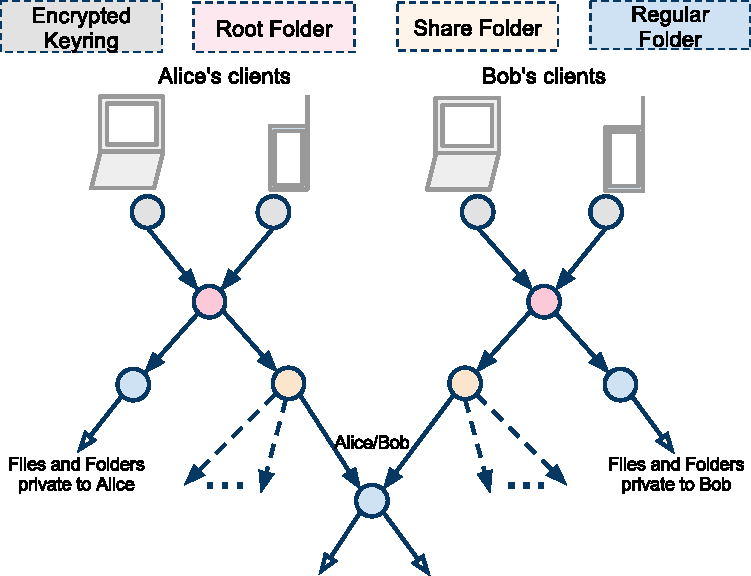
\includegraphics[width=\columnwidth]{ArchitectureFileSystem.pdf}
    \caption{File System Structure}
    \label{fig:AS:filesystem}
\end{figure}

The file and directory structure can be seen as a directed graph, as illustrated
in Figure \ref{fig:AS:filesystem}, and users can link in folders and files as
wanted. This provides a flexible and space-conservative structure that is easily
extendible.

Each client\footnote{I.e. the different user terminals.} keeps a local copy of
the identity and write key to the users root folder in a password
protected keychain. In the event of loss of one of the clients, a user can change
encryption keys (and identifier) for the root folder, and hence effectively
block out the compromised clients.

\begin{table}
  \centering
  \caption{The structure of a folder entry}
  \begin{tabular}{ | l | l |}
    \hline
    \textbf{Data}       & \textbf{Comment}                          \\ \hline
     Alias              & Human readable name of file/folder        \\ \hline
     Storage Index      & Key to retrive file/folder from server    \\ \hline
     Write Capability   & Only for folders, needed to write a file  \\ \hline
     Read Capability    &                                           \\ \hline
     Verify Capability  & Only for folders, needed to verify a file  \\ \hline
  \end{tabular}
  \label{tbl:folder:contents}
\end{table}


A directory contains two types of data. It contains meta data about it self and
in addition zero or more entries. Table \ref{tbl:folder:contents} exhibits the
structure of the folder entries. The \emph{Alias} field is the name of a
specific child. The \emph{storage index} is the look-up value of the
corresponding child.

The meta data are described in Table \ref{tbl:folder:meta}. The \emph{Storage
Index} is a unique value derived from a directory's read key and serves as an
identifier for the directory in question. The other elements are used for
security purposes, and are described further in Chapter \ref{chap:CS}.

\begin{table}
  \centering
  \caption{Meta data for a directory}
  \begin{tabular}{ | l | l | l | l | l | l |}
    \hline
    Public Key & Storage Index & \acs{IV} & Write Enabler &  Signing Key  &  Signature  \\ 
    \hline
  \end{tabular}
  \label{tbl:folder:meta}
\end{table}


\section{ACL/Authentication Layer}

There should be some layer present on the application which enforces \ac{ACL}s
and authenticates users which should have access to the stored files. From a
security standpoint this is not necessarily required. An attacker would have to
be able to guess the storage index\footnote{Or the ``key''} and the
corresponding encryption key for that index to be able to get any information
out of the system. But there are however several reasons why we believe this
layer should be implemented, as per described in the following sections.

\subsection{Block access}
If for whatever reason a storage index and corresponding decryption key is
leaked to some third-party, but not to the cloud provider, the layer can
prevent an unauthenticated user from retrieving the file. The possibility of
also denying authenticated users from retrieving files is also a wanted feature
for instance in the event of a stolen/lost terminal where the credentials are
saved.

\subsection{File Deletion}

The way of the proposed solution to handle folders, allows a distinction between write
access and read access. The write key can be used to deduce a secret that can
be safely leaked to the server which in turn would be used decide if a user has
permission to delete a folder. It could also be used for deciding if a user has
permission to write to files, but this can be verified by the server in terms
of the signature.

For immutable files there is no concept of write-access, only read. It is both
illogical and impractical to assume that read access should also yield
delete access. A layer which identifies which users first creates a file, can by
the same method decide who should be able to delete a file. 

\subsection{Accounting}

If this application were to by run by a cloud storage provider, it is
important to be able to decide which person should be billed for the storage of
files, as well as the traffic generated by users uploading and downloading
files. 

For an immutable file, this can be identified by the user who created the file,
and the traffic is billed on whoever retrieved or uploaded the file.

Accounting might also be interesting for an organization using a third party
cloud provider. For instance an employee who leaves the organization might be
tempted to copy all the data stored on the server, the organization should then
be able to discover what he has done. It is however worth noting that if the
accounting happens server side, there is no real way to verify that all logs
stored there are correct, since the cloud provider will have access to at least
delete them.

\section{User scenarios}

The various user scenarios the software has to support, provides a logic way to
describe the external properties of the system. The fundamental operations are
\emph{downloading}, \emph{uploading} and \emph{sharing} of files.

\subsection{Download file}

When a user wishes to download a file or directory, all that is needed is the
password to unlock the local keychain on the user terminal, as depicted in Figure
\ref{fig:AS:download}. The client sends a GET request with the identifier in
question, and the server responds with the encrypted folder. This contains the
capabilities needed to locate and decrypt the underlying files and folders.
After decrypting the contents, the client again queries the server with the
identifier of the wanted file, and there after decrypts it, before displaying it
to the user.

\begin{figure}[h!]
    \centering
    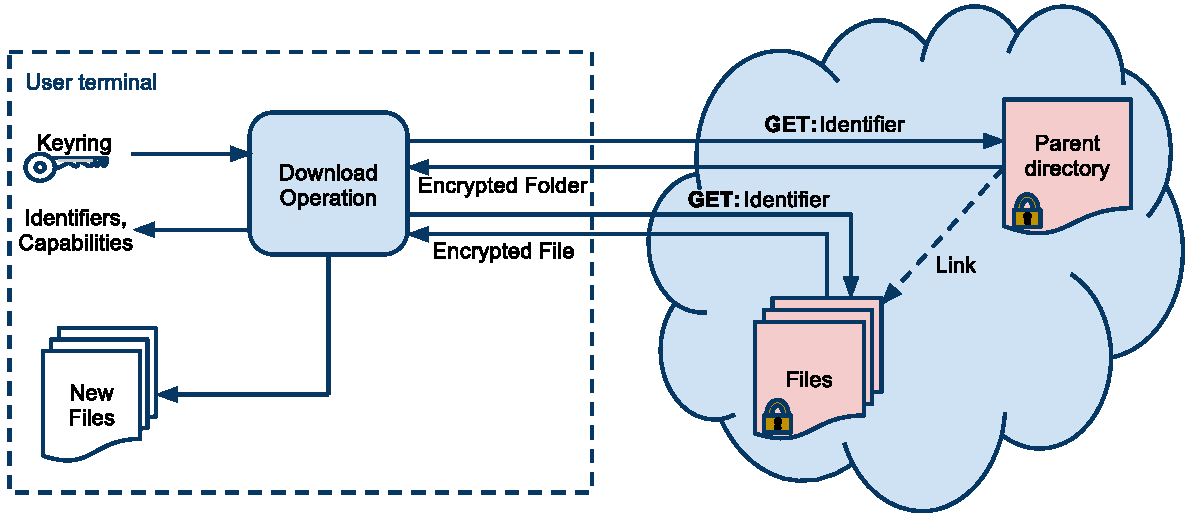
\includegraphics[width=\columnwidth]{ArchitectureDownload.pdf}
    \caption{Scenario: Downloading of files}
    \label{fig:AS:download}
\end{figure}

\subsection{Upload Files}

Figure \ref{fig:AS:upload} shows the process of uploading new files. The only
information the server in the cloud receives, are identifiers and encrypted
containers. The user is also given the opportunity to transfer the corresponding
identifiers and capabilities to other users.

\begin{figure}[h!]
    \centering
    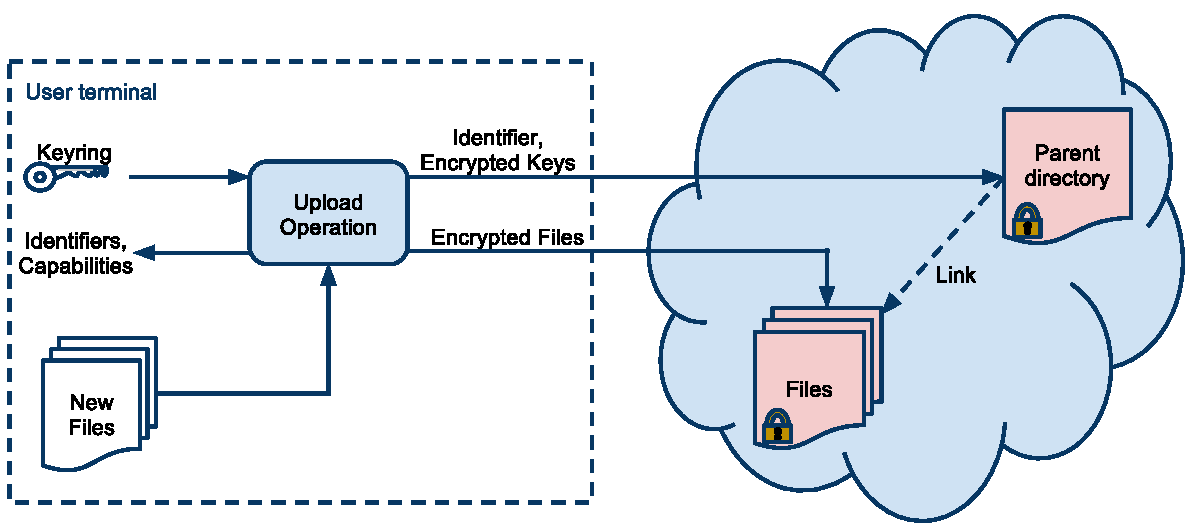
\includegraphics[width=\columnwidth]{ArchitectureUpload.pdf}
    \caption{Scenario: Uploading of files}
    \label{fig:AS:upload}
\end{figure}

Before uploading, the client has to find, download and decrypt the directory the
files are to be placed in. This process was described in the previous section.
The cryptographic details of the Upload Operation can be found in Section
\ref{sec:CS:UF}.

\subsection{Share files}

As shown in Figure \ref{fig:AS:sharing}, for Alice to be able to share files
with Bob, she first has to create a new directory. After the capabilities to
this directory has been shared with Bob, this directory is going to be the
secure channel where they can share folders and files.

Before transferring the capabilities to Bob, Alice links the shared directory to
a parent directory, so she can easily find it again at a later time. She can
also link files to the shared directory.

\begin{figure}[h!]
    \centering
    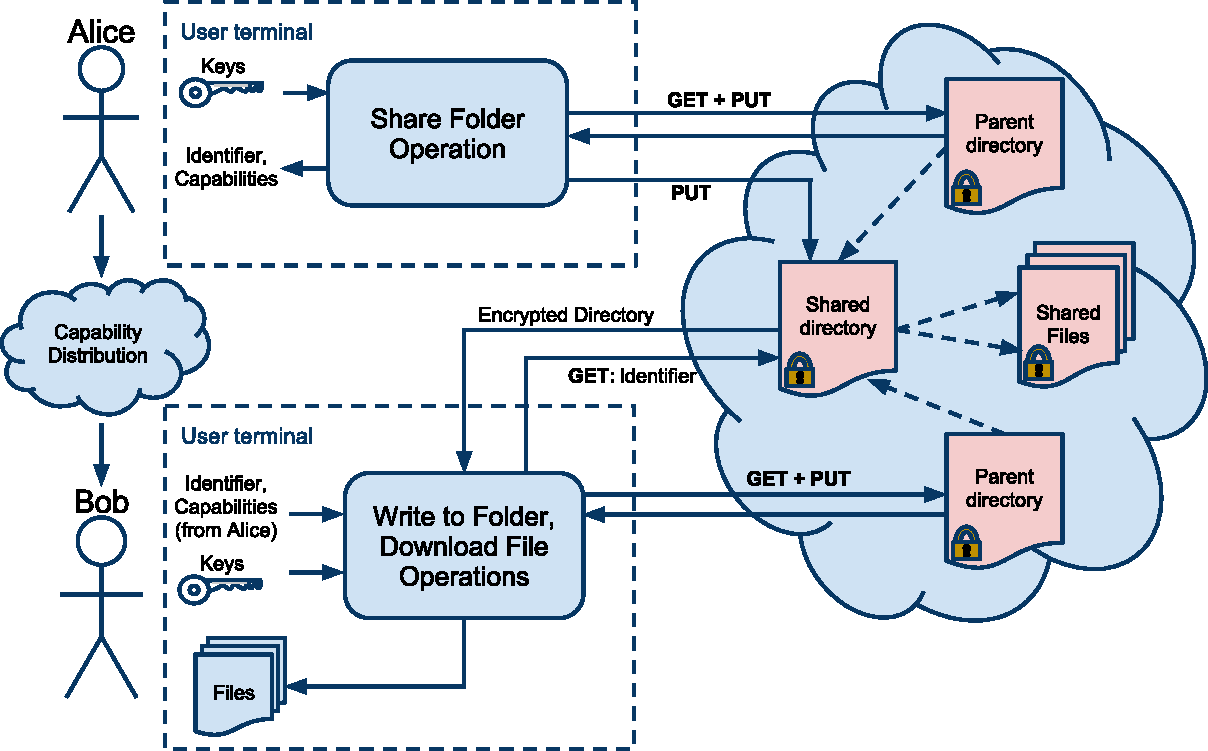
\includegraphics[width=\columnwidth]{ArchitectureShare.pdf}
    \caption{Scenario: Sharing files}
    \label{fig:AS:sharing}
\end{figure}

The capability distribution is a key design issue, and has to be performed in a
secure manner. This can be solved in a variety of ways, and the solutions
proposed in this thesis will be described in Chapter TODO.

After receiving the capabilities for the shared folder from Alice, Bob requests
and receives the encrypted shared directory, in addition to linking it with a
parent directory for future usage. He can then download shared files as if they
where his own.

\paragraph{Read-Only shares.}

If Alice wants to share a directory in Read Only Mode with Bob, she can simply
not include the write capability in the parent directory. This will work as
intended until Alice wants to write to the folder, thus the write capability has to
be stored another place. We will implement this as a special folder under the
root folder, and link in all such folders and files the ``normal'' way here.
This process is illustrated in Figure \ref{fig:AS:readonly}.

\begin{figure}[h!]
    \centering
    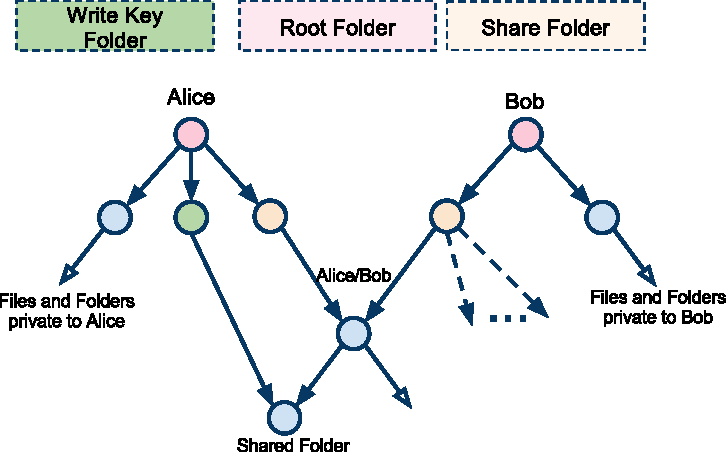
\includegraphics[width=\columnwidth]{ArchitectureShareReadOnlyFolder.pdf}
    \caption{Sharing write-protected folders}
    \label{fig:AS:readonly}
\end{figure}

\section{Implications of User Equipment}

The software should be able to run on restricted devices, i.e. equipment with
limited memory and \ac{CPU} power, often in addition to constraints on power and
network consumption.

This has implications for the design of the software, since all cryptographic
operations has to be performed client-side. These considerations will be
brought up throughout the further description of the software.

%**************************************%
\chapter{Cryptographic Architecture}
%**************************************%
\label{chap:CS}
This chapter will elaborate on the cryptographic solutions applied to the
architectural scheme in Chapter \ref{chap:AS}. We will take a closer look at
how confidentiality, integrity and authentication can be integrated into the
proposed architecture.

%A fundamental scheme for key distribution is needed to realize the desired
%security features, hence an appropriate solution for key distribution will
%also be given.

The first section is a brief introduction explaining the basic
security concept used by the application. Following is a detailed description of
the cryptographic solutions adapted. The cryptographic solutions are revealed
in terms of file and directory operations performed by the application. The
chapter ends with a description of a users keychain.

\section{Security Concept}

The basic security concept of the application is to keep a user's remote storage
confidential to a third-party storage provider. To solve this, the application
encrypt files locally at the users terminal before uploading them to the
third-party storage provider. When accessing a file, the application first
download the encrypted file and further decrypt it locally. To enable this
simple encryption scheme, the user terminal is required to possess at least one
cryptographic key. Cryptographic keys are stored in a single keychain at the user
terminal.

By initially knowing that files are placed encrypted on a remote server and that
the local user possess one or more cryptographic keys, we can continue with a
more comprehensive description of the complete cryptographic solution. The
details are explained in terms of the following directory and file operations.

\section{Directory operations}
\label{sec:CS:DO}

This section presents the two basic directory operations used by the
application. The ``create directory'' and ``open directory'' operations are
explained as follows.

\subsection{Create Directory}

The create directory operation is divided into two subsequent parts. First, the
directory must be created locally at the user's terminal. Second, the directory
must further be uploaded to the remote server.  Uploading a file or directory is
possible only if the user is authenticated.

Creating and uploading a directory from the user terminal is illustrated in
Figure \ref{fig:CS:CD}.

\begin{figure}[h!]
    \centering
        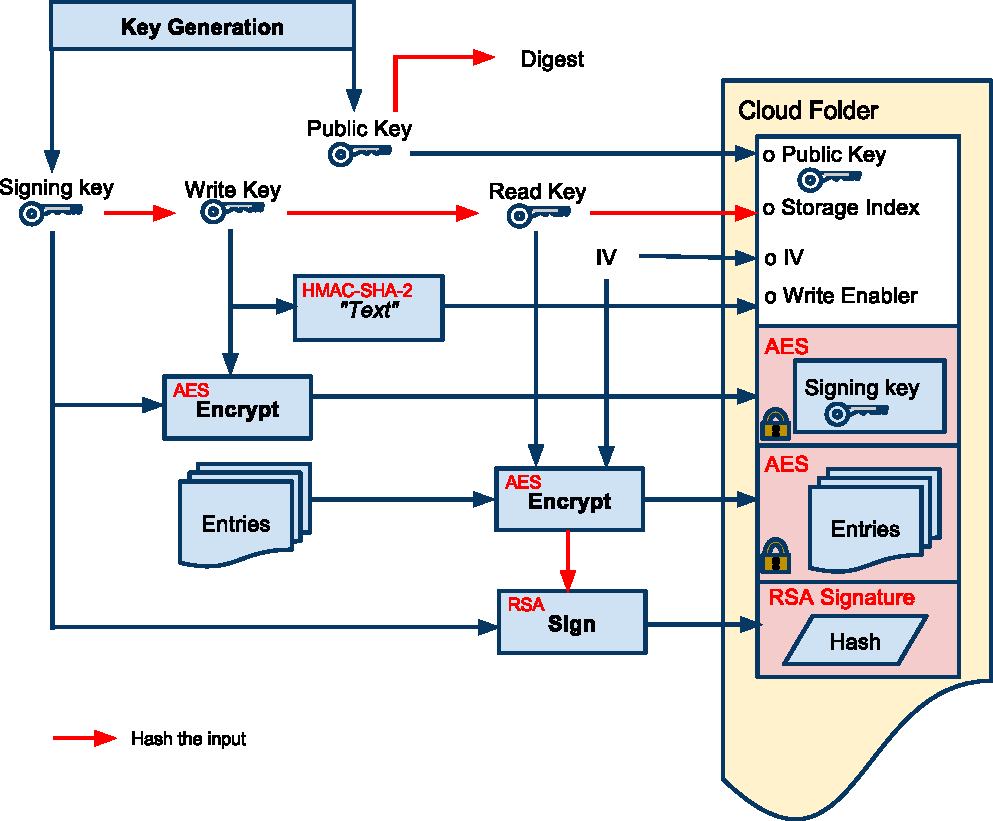
\includegraphics[width=\columnwidth]{CryptoCreateFolder.pdf}
	    \caption{Creating and uploading a directory.}
    \label{fig:CS:CD}
\end{figure}

Before creating a new directory it is necessary to generate an RSA key-pair. The
key-pair is specific to the new directory and consists of a public and private
signing key. The signing key is further used to derive a write and a read key
for the corresponding directory. The read key is a hashed value of the write
key, while the write key equals the hashed value of the signing  key. 

% TODO: Will we use counter IV?
After key generation, the public key is directly added to the new directory. The
directory's storage index is further added as a hash value of the directory's
read key. The next value added to the directory is the initialization vector
\ac{IV}. The IV is generated from a counter value stored at the user terminal. It
is used to prevent predictable ciphertext, when the directory's entries are encrypted.

The next value added to the directory is the write enabler. The write enabler is
an HMAC-SHA-2 value created from the directory's write key and a static chosen
text value. It is uploaded as a part of the directory, but can never be
downloaded from the server. The write enabler is used by the server to enable
users, that possess the directory's write key, to modify the directory. This
ensures that only authorized users can modify a directory.

After adding the write enabler, the user must add the directory's private
signing key. The signing key should only be available for users with write
permission to the directory. It is therefore encrypted with the directory's
write key before it is added to the directory. The signing key is encrypted using \ac{AES} in
\ac{CBC} mode. The next value added is the directory's entries. The entries of a
directory should only be visible to users with read permissions to
the directory. They are therefore encrypted with the directory's \ac{IV} and read
key prior to insertion. The entries are encrypted using \ac{AES} in \ac{CBC} mode. The
last value added to the directory is a signed hash value of the encrypted
entries. The hash value is encrypted with the signing key using \ac{RSA}. A
signature is needed for other users to know that the directory was created from
an authorized user.

After creating a new directory, the directory is further uploaded to the remote
server.

It is important to notice that none of the values contained within the
directory or any of the cryptographic keys are kept locally by the user. The
user can only achieve the public and private keys through the remote directory.
The directory's read and write keys can only be achieved through capabilities stored
in the remote directory's parent directory. This is true for all directories
stored on the server except for the user's root directory. The keys to the
root directory are stored in the user's local keyring. The keyring is explained
in Section \ref{KEYRING}.

\subsection{Open Directory}

This section describes the procedure for opening a directory. Opening a
directory involves both downloading, verifying and decrypting the directory. The
download and verify procedure is illustrated in Figure \ref{fig:CS:VOD} and
described below. A description of the subsequent decryption procedure follows.

\begin{figure}[h!]
    \centering
    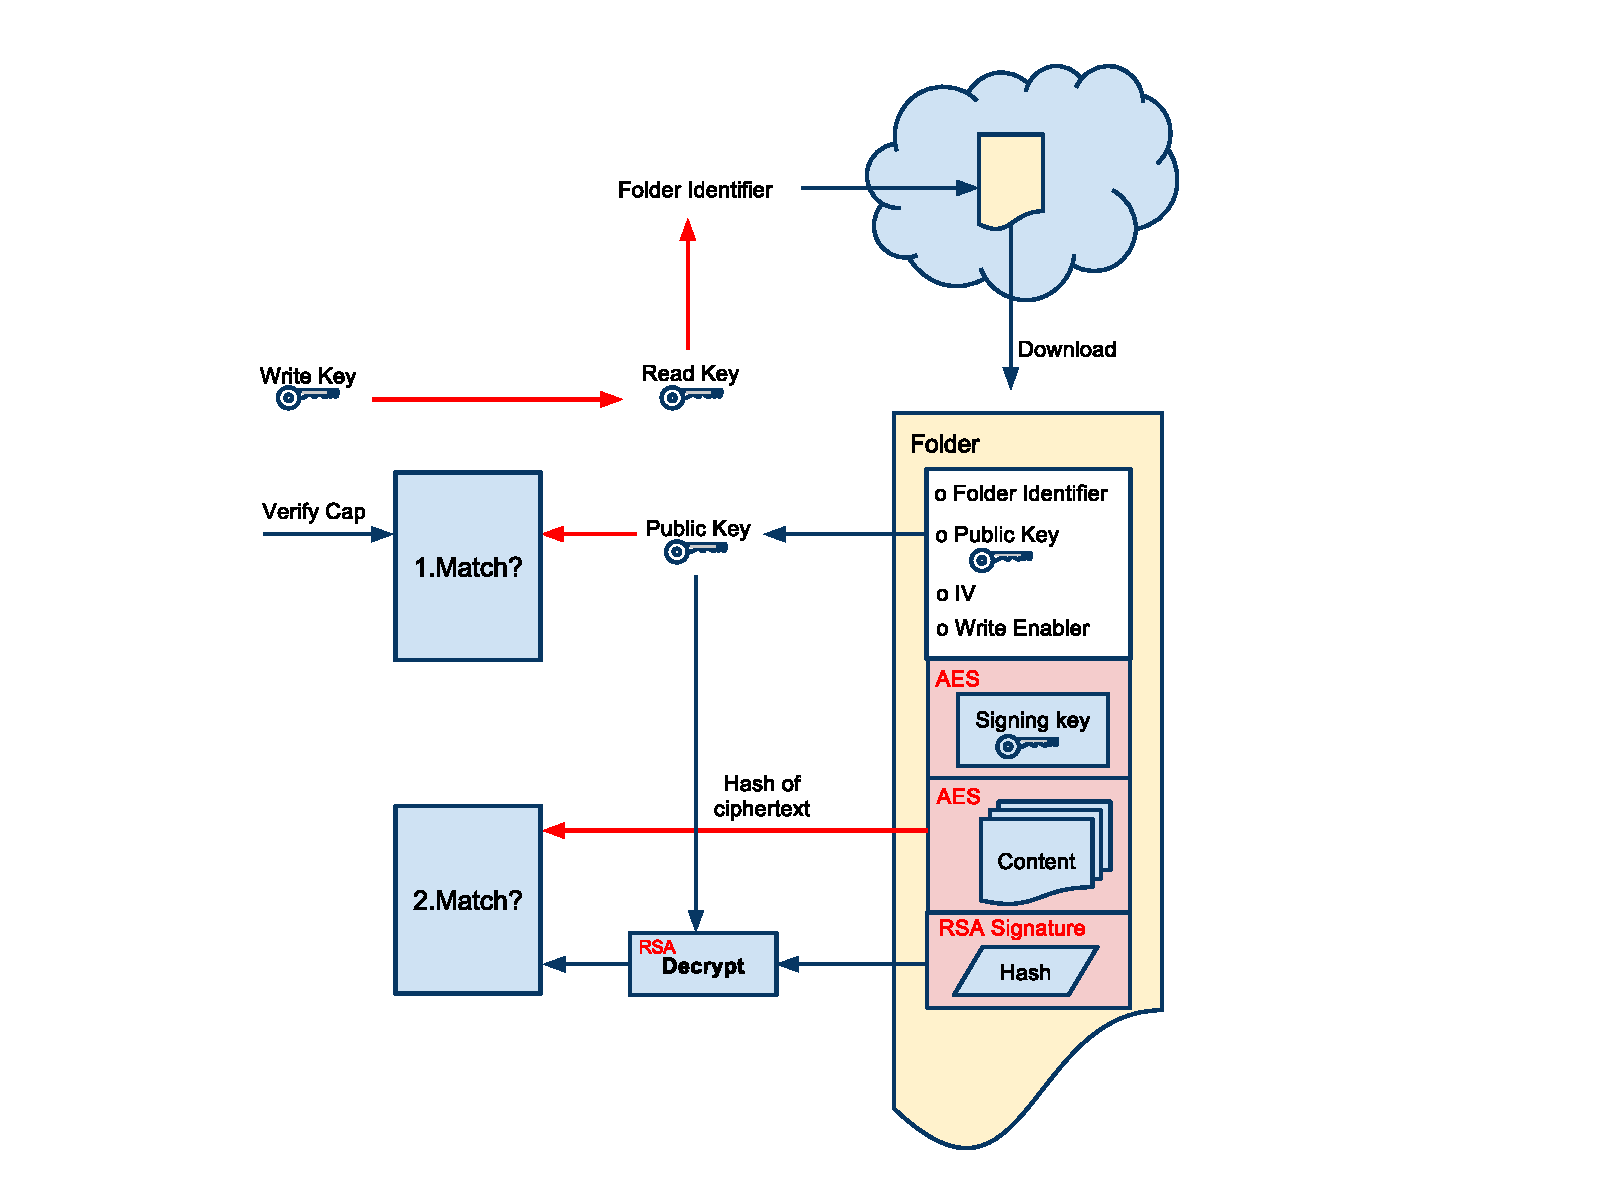
\includegraphics[width=\columnwidth]{VerifyOpenFolder.pdf}
    \caption{Downloading and verifying a remote directory.}
    \label{fig:CS:VOD}
\end{figure}

First of all, to download a desired directory, the user must be in
possession of a read key specific to that directory. The read key is either
created from a hash value of the directory's write key, or obtained from a read
capability stored in the parent directory.

The directory's storage index is further obtained. It is either created from the
obtained read key, or obtained from the read capability stored in the parent
directory. The storage index is a simple hash value of the read key. It is used to
localize the specific directory on the remote server. The localized directory is
further downloaded to the user's terminal.

When the correct directory is downloaded, it will further exhibit a verification
procedure prior to decryption. The verification procedure is illustrated in
Figure \ref{fig:CS:VOD}.

The purpose of the verification procedure is to check the integrity of the
content and to verify that it has been written by an authorized user.
If one or neither of these checks are verified, the directory content will not
be decrypted.

The first check verifies the correctness of the public key stored within the
downloaded directory. The key must be checked to ensure that it belongs to the signing
key. If it does, it indicates that an authorized user has signed the directory
content. The check is carried out by hashing the directory's public key and
comparing it with a verification capability.

If the directory passes the first check, it will further be checked for content
integrity. The integrity check ensures that the directory content, in form of
entries, has not been tampered with. It is carried out by decrypting a stored
encrypted hash value in the directory and comparing it against the hash value of
the directory's encrypted entries. The encrypted hash value stored in the
directory is decrypted using the previously verified public key. The integrity
check is depicted as a part of Figure \ref{fig:CS:VOD}.

If the directory passes the verification procedure, the user will decrypt the
directory's encrypted entries using the directory specific read key. The decryption procedure
is illustrated as a part of Figure \ref{fig:CS:OD}. An \ac{IV} is additionally
used with the read key to carry out the decryption procedure. The \ac{IV} is easily
fetched from the directory prior to decryption.

\begin{figure}[h!]
    \centering
    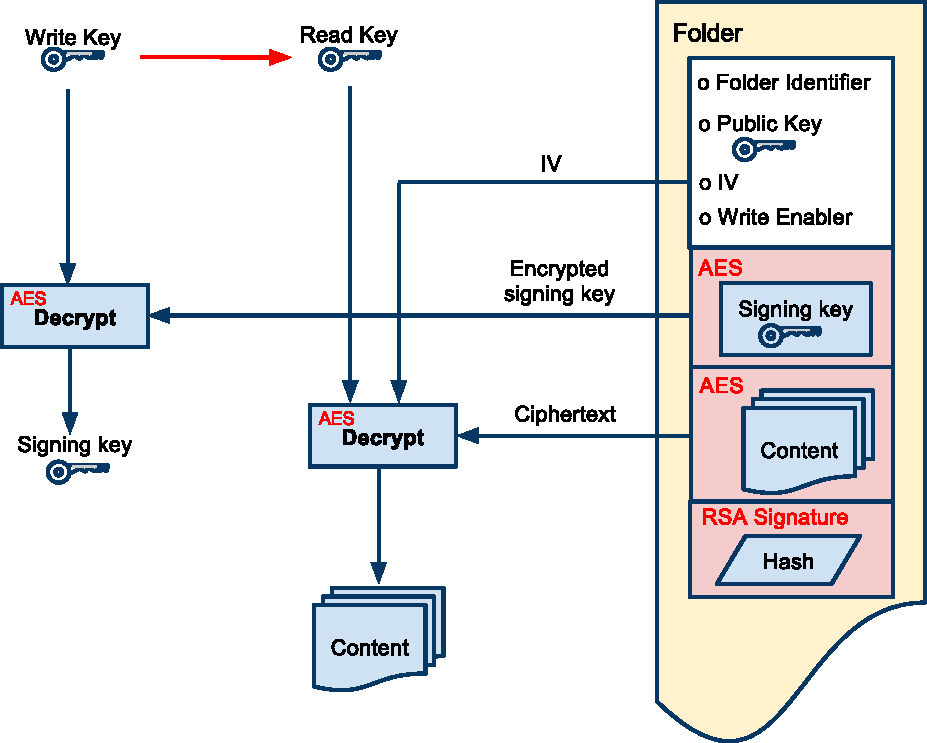
\includegraphics[width=\columnwidth]{OpenFolder.pdf}
    \caption{Decrypting a remote directory: Decrypting directory content and
    obtaining the signature key.}
    \label{fig:CS:OD}
\end{figure}

\subsection{Modify directory}
In addition to read the content of a directory, the user might want to write to it as well. 
To be able to modify a downloaded directory, the user must be in possession of
the directory's write key. The write key is needed to obtain the directory's
signing key and write enabler. 

The signing key is needed by the user to correctly sign the
modified directory. Remember that a directory can only be read by users if it
contains a valid signature. Obtaining the signing key from a downloaded
directory is shown as a part of Figure \ref{fig:CS:OD}.

The write enabler is generated as a HMAC-SHA-2 value from the write key and a
static known text value. It is used to prove the user's write permissions to the
receiving ACL layer at the remote server. This ensures that the directory has
been modified by an authorized user.

The user fetches the encrypted signing key and decrypts it with the
write key. This is illustrated in Figure \ref{fig:CS:OD}.


\section{File Operations}
This section describes the elementary file operations supported by the 
application. The ``create file'' and ``open file'' operations are considered.

\subsection{Create File}
In the create file operation, a file must be created locally on the user's terminal
prior to upload. The operation is depicted in Figure \ref{fig:CS:CF} and
described as follows.

\begin{figure}[h!]
    \centering
    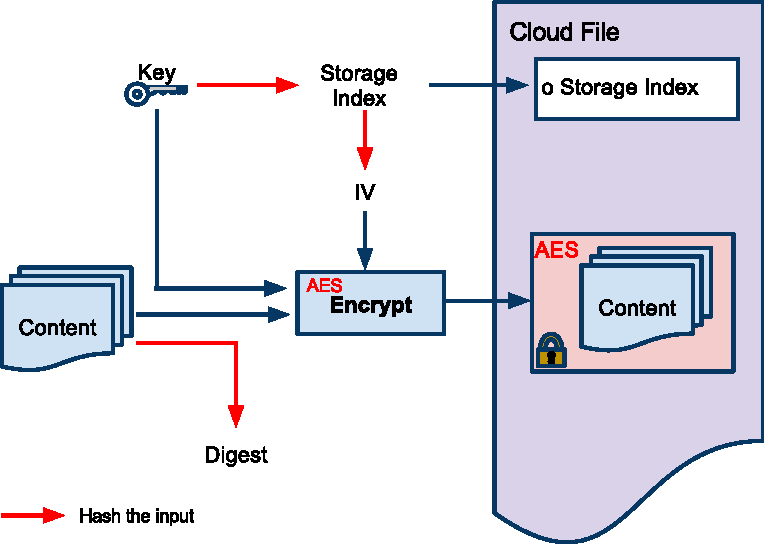
\includegraphics[width=\columnwidth]{CryptoCreateFile.pdf}
    \caption{Creating and uploading a file. }
    \label{fig:CS:CF}
\end{figure}

The user chooses a local file to upload. This file is depicted as the
``content'' value in Figure \ref{fig:CS:CF}. A cryptographic write key, specific
for the new file, is further generated. The key generation algorithm is
explained in Section \ref{KEYGEN}. The write key is further hashed to create a
file specific storage index. The storage index is stored in the new file. A
file's storage index has the same property as a directory's storage index. The
\ac{IV} is the next value that is inserted into the new file. It is
generated from a counter stored at the user's terminal.

The previously chosen file content is further encrypted with the write key and
file \ac{IV}. The encrypted file content is then inserted to the new file. The last
value added to the new file is an encrypted hash value of the encrypted content.
The hash value is encrypted using the file's write key. Both the file content
and hash value are encrypted using \ac{AES} in \ac{CBC} mode.

\subsection{Open File} 
\begin{figure}[h!]
    \centering
    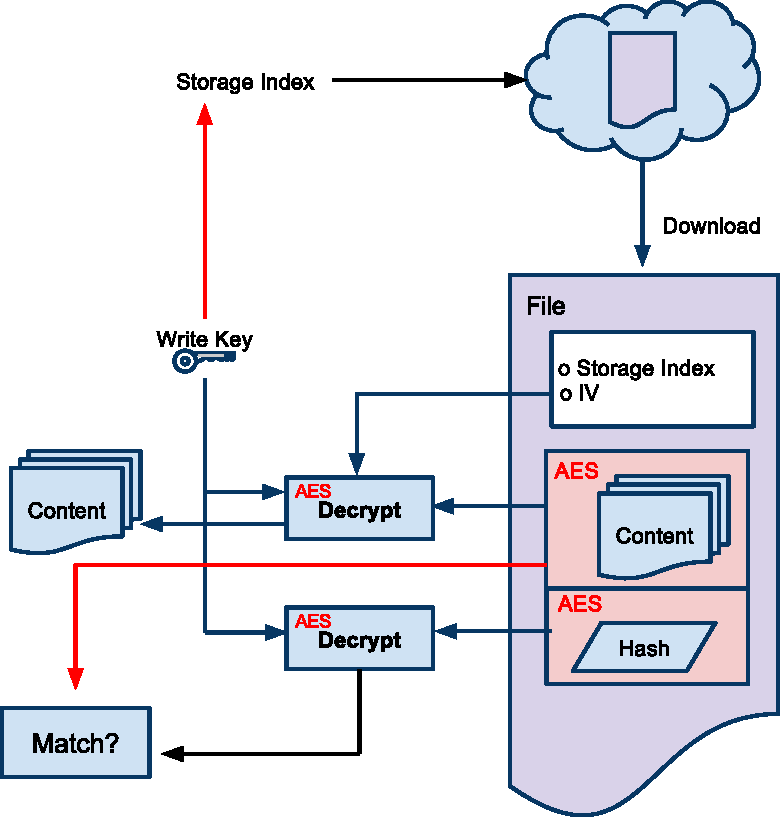
\includegraphics[width=\columnwidth]{CryptoOpenFile.pdf}
    \caption{Downloading a file from the server}
    \label{fig:CS:OF}
\end{figure}

The process of retrieving a file is illustrated in figure \ref{fig:CS:OF}.A
file is located by hashing the write key, which in turn is obtained either by
knowledge by the user or client or from a parent folder. The ciphertext, the
\ac{IV} and the encrypted hash of the ciphertext is downloaded from the server.
The ciphertext is hashed client side and the encrypted hash from the server is
decrypted with the write key, if these two outputs match the ciphertext has not
been tampered with. The ciphertext is then decrypted using the write key and
\ac{IV} to obtain the file contents.

\section{Keychain}

As stated, each client keeps a local copy of the identity and write key to the
personal root folder in a password protected keychain. This is done to be able
to encrypt the root folder with a key that is not based on a password, but
completely randomly generated. In addition, this means that no special scheme is
needed for the root folder, as we can use the same procedures as for ``normal''
folders as defined in the previous sections.

The strength of a password is related to its length and its randomness
properties. Passwords shorter than 10 characters are usually considered to be
weak \cite{pbkdf_nist}. In the event of loosing one of the clients, and thus the
keychain, a potential attacker can use fast password cracking attacks to try to
compromise the root folder keys. As an precaution for this, we will use
\ac{PBKDF2}/RFC2898\footnote{http://tools.ietf.org/html/rfc2898} with a salt
value to create additional computational work for the process of unlocking the
keychain. This method is known as key stretching \cite{keystretch}.



\section{Choice of cryptographic primitives}
The scheme which has been described in this section requires three primitives;
a cryptographic hash function, a symmetric cipher and an asymmetric cipher
which can be used for digital signatures. The choices should reflect the
following security demands of our application, all with the assumption that the
possible attacker has access to vast quantities of computing power.

% TODO: Sikkerhetskrav bør vi definere tidligere
\begin{enumerate}
    \item It should be infeasible to break confidentiality for any file or folder
    \item It should be infeasible to break integrity for any file or folder
\end{enumerate}

\subsection{Symmetric Cipher}
For a symmetric cipher the choice is pretty simple; \ac{AES}. \ac{AES} is
a standard, has been around for a long time, and does not have any serious
security issues as long as it is used correctly.
% Kilder kilder TODO

%**************************************%
\chapter{Implementation}
%**************************************%
This chapter describes the implementation of our proof-of-concept client and
server. The technologies and software \ac{API}s used will be described, in
addition to implementation details that require special attention.

\section{Server}

The server, in the most basic form, has to support two operations -- sending
and receiving files. In addition, an \ac{ACL} layer is needed to support user
management and access control to able to allow the deletion of files from the
server.

\subsection{Communication and Architectural Patterns}

By definition, cloud applications are accessible over the Internet. The system
we are creating, should be able to send and receive files and information from
a server in the cloud. The \acf{HTTP} is the foundation of data communication
for the World Wide Web, it is well tested, will pass through most firewalls and
has a multitude of libraries in programming languages. To get a working server
we can also use any existing web server as a foundation, which saves a lot of
work. Thus \ac{HTTP} was chosen as our communication protocol.

\subsubsection{\acs{REST}} The Web is built around an architectural style called
\ac{REST} \cite[ch. 5]{fielding}, which is defined by four interface
constraints: identification of resources, manipulation of resources through
representations, self-descriptive messages, and, hypermedia as the engine of
application state. In addition, \ac{REST} dictates five\footnote{And one
optional, Code on demand, which is not applicable for our system.} architectural
constraints \cite{fielding}. Our server application adheres to these
constraints or \emph{patterns} as follows:

\begin{description}
  \item[Client-server] \hfill \\
    The server is our server application, and the client is the various client
    applications, 

  \item[Stateless] \hfill \\
    Since the server is just a simple key-value file store, it does
    not need to keep state.

  \item[Cacheable] \hfill \\
    The server could easily add caching, by putting each encrypted file in
    memory as downloaded, and using the Least-Frequently Used algorithm for
    choosing which items to swap out. In addition, for every update of a folder,
    the corresponding cache item has to be marked as invalid.

  \item[Layered system] \hfill \\
    Layers are used to encapsulate, separate and hide functionality.
    Figure \ref{fig:IM:layers} illustrates the layers of the server application.

  \item[Uniform interface] \hfill \\
    The interface between clients and server(s) are given by the URI scheme in
    Table \ref{tbl:IM:restinterface}. When a folder is uploaded a Write Enabler
    must also be provided together with the storage index..
\end{description}

\begin{figure}[h!]
    \centering
    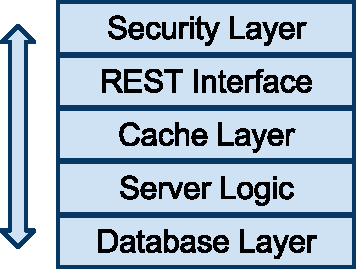
\includegraphics[scale=0.6]{ImplementationServerLayers.pdf}
    \caption{Architectural Layers in the Server application.}
    \label{fig:IM:layers}
\end{figure}

\begin{table}[h!]
    \centering
    \caption{The \acs{REST} interface of the server application.}
    \begin{tabular}{|l|l|}
        \hline
        \multicolumn{1}{|c}{\textbf{\acs{URI}}} & \multicolumn{1}{|c|}{\textbf{Description}} \\
        \hline
        \texttt{/put/<storage index>} & Creates or updates encrypted file \\
        \hline
        \texttt{/get/<storage index>} & Retrieves encrypted file \\
        \hline
    \end{tabular}
    \label{tbl:IM:restinterface}
\end{table}

In this context, resources are the encrypted files, and the architectural
constraints of \ac{REST} also matches that of our system as a
whole. Thus, the server application are designed in a \acs{REST}ful manner.

\subsubsection{Network Security} Since we are utilizing \ac{HTTP}, we can
easily add an extra layer of \ac{TLS} to form \ac{HTTPS}. This makes it more
difficult for potential attackers to intercept messages, and also provides
protection against the most basic form of \ac{MITM} attacks. It also provides
protection against eavesdropping, which would have revealed the Write Enabler
for folders and could be used by an attacker to delete user files. The top-most
layer of Figure \ref{fig:IM:layers} thus refers to \ac{TLS}.

\subsection{Environment}

The Python programming language in a Linux environment was chosen as development
platform, together with a set of applications, interfaces and micro frameworks.
The rationale for each of these follows.

\paragraph{Python} Python is a high-level general-purpose programming language.
It was chosen due to previous knowledge and experience by the
authors, in addition to its simplicity.

\paragraph{Apache} The Apache HTTP Server is a well tested and used web
server. According to \citet{netcraft}, Apache is by far the most used web server
software, and has been so since 1996. It was chosen on the basis of previous
experience and its superb documentation.

\paragraph{\acs{WSGI}} The Python \ac{WSGI} is, as the name suggests, an
interface between a web server and a Python application. It is defined in
\ac{PEP} 3333\footnote{\url{http://www.python.org/dev/peps/pep-3333/}}, and
specifies both sides of the interface -- the \emph{application} and the
\emph{server}. The server side is implemented in the form of an Apache 
module, namely \texttt{mod\_wsgi}, and the application is where we put our
code.

For each of the requests the server (i.e. \texttt{mod\_wsgi}) receives, a call
to the application function is made with two arguments -- a data structure
containing the environment variables, and a callback function for which the
application uses to return data to the requesting user via the server.

\paragraph{Pyroutes} To adhere to the \ac{DRY} principles, we chose to make use
of a micro framework around \ac{WSGI} called
Pyroutes\footnote{\url{http://www.pyroutes.com/}}. It provides shortcuts for the
most frequently used functionality when developing web services, as that of
\ac{URL} handling and processing of submitted user data in the form of
\texttt{GET} and \texttt{POST} requests.

Pyroutes did not, however, support the HTTP \texttt{PUT} request, so this was
implemented and contributed back to the project.

\subsection{Implementation Details}

The code was structured as illustrated in Figure \ref{fig:IM:layout}. The file
\texttt{handler.py} provides the interface for \texttt{mod\_wsgi} and the server
application, and basically includes the \ac{URL} scheme in
\texttt{fileserver.py}. An example \ac{URL} mapping is shown in Listing
\ref{lst:IM:get}. The function \texttt{get\_file} is registered to have the
\ac{URL} \texttt{/get} through the decorator provided by Pyroutes. After
retrieving the file from disk, a proper \ac{HTTP} response is returned,
containing required headers.

The file \texttt{filesystem.py} contains the low-level file system operations,
\texttt{save\_file()} and \texttt{retrieve\_file()}, together with a set of
helper functions to manage file access checking and database operations.  The
folder \texttt{sql/} contains \ac{SQL} code to create necessary tables in the
database, and \texttt{db.py} provides an helper function to connect to the
database.

\begin{figure}[h!]
\begin{verbatim}
|-- cloudstorage
|   |-- __init__.py
|   |-- db.py
|   |-- fileserver.py
|   |-- filesystem.py
|   |-- settings.py
|   `-- sql
|       `-- write_enablers.sql
|-- handler.py
`-- tests
    `-- filesystem_tests.py
\end{verbatim}
    \caption{Server module structure}
    \label{fig:IM:layout}
\end{figure}

\lstinputlisting[language=Python,breaklines=false,label=lst:IM:get, caption=URL mapping in fileserver.py]
{listings/fileserver.py}

\subsubsection{\acs{ACL} functionality}

The only \ac{ACL} functionality implemented, is the server-side verification
that a client has proper access to overwrite a file, e.g. when a client wishes to
update a folder with new contents. We call this \textbf{Write-Enabler Verification}. 

When a client first uploads a new folder, it also provides a
\emph{Write-Enabler Key}, which the server adds to the database along with the
\emph{Storage Index} of the folder.  For every subsequent request to write to a
file with this specific Storage Index, the server verifies that the provided
Write-Enabler Key is equal to that in the database.

If a client tries to put a file with a Storage Index that already exists, the
server replies with an error code if the client in addition does not provide a
valid Write-Enabler Key.

\section{Client - Android}
% Java/Android/Dalvik/JCE/Commons HTTPClient
% Security vs. Usability - Rationale for GUI
% MVC? V=Android GUI
%
The \ac{PoC} client we have implemented, is made for devices using the Android
operating system, which is based on Linux. The \ac{SDK} for making Android
applications, is essentially a somewhat modified version of Java. 

Most devices that use the Android operating system are mobile phones or
tablets, which implies that they are limited in terms of speed and
memory. The point of making the \ac{PoC} client for such a device, i.e. a
\emph{smart phone}, is the growing availability, and the flexibility these
devices provide. A user carries the device everywhere, it has a network
connections, and it is always on.

A nice side effect of developing on a smart phone platform, is that if the
software performs well on a constrained device, it will almost certainly also
have good performance on any faster device as well. 

\subsection{Environment}
The \ac{PoC} client was made on the Android platform in the Java programming
language, together with a set of frameworks. The rationale for these are as
follows.

\paragraph{Android} The Android operating system is made by Google, and is most
commonly found on mobile phones and tablets. The platform choice of Android was done
based on hardware availability and familiarity with developing on the
platform and the programming language (Java). 

\paragraph{Java} Java is a high-level, object-oriented programming language.
Applications written in Java runs in a \ac{JVM}, which implies that a Java
application can run on almost any device which has a \ac{JVM}. The \ac{JVM} on
Android is called Dalvik.

\paragraph{HttpComponents} Apache HttpComponents are a set of libraries for
\ac{HTTP} transport in Java. The part used in our client is called HttpClient.
Android incorporates parts of this client in its native \ac{JVM}. The use of
this library adheres to the \ac{DRY} principles.

\paragraph{\ac{JCA}} \ac{JCA} is an architecture for doing cryptographic
operations in Java. The architecture is based on principles of implementation
independence, implementation interoperability and algorithm extensibility.
Basically what this means, is that each implementation of the \ac{JVM} can have
different implementations of the cryptographic primitives, but the developer
does not need to know which implementation is available.

\paragraph{ZXing Barcode Scanner} ZXing Barcode Scanner is a popular Android
application which can be used by other Android applications to both scan and
generate barcodes. By the use of this application, we adhere to the \ac{DRY}
principles, by not creating our own code to generate barcodes.

\subsection{Architectural Patterns}

\paragraph{Client-server} It should be obvious that the client we have
implemented is the client part of the overall client-server pattern.

\paragraph{Pipe-and-Filter} The basis of the pipe-and-filter pattern is that
there exist a chain of processing elements, where the output of one element is
the input of the next element. We use this for file uploads and downloads to
limit the memory usage of the client, as well as to increase performance.

\paragraph{Asynchronous pattern} We use asynchronous calls to slow operations
-- e.g. file upload and key generation -- extensively, to prevent the interface
from hanging and to deliver a smoother user experience in general.  

\subsection{Implementation Details}

\subsubsection{Structure}
% Package Structure, some nice UML (?)
% Which qualities do we wish to achive? Security, Performance, Usability
 
The source of our client is logically separated into two entities --
\textbf{CSVlib} and \textbf{CSVAndroid}. CSVlib is a pure Java library which
contain the necessary entities, cryptographic operations and communication
calls required for the client. CSVAndroid contains primarily a graphical user
interface to make use of CSVlib on an Android device.

\subsubsection{Cryptographic Entities}
All the cryptographic entities -- namely folders, files and capabilities -- are all
part of CSVlib. Their relationship can be seen in Figure \ref{fig:CSVlib:overview}.

\begin{figure}[h!]
    \centering
    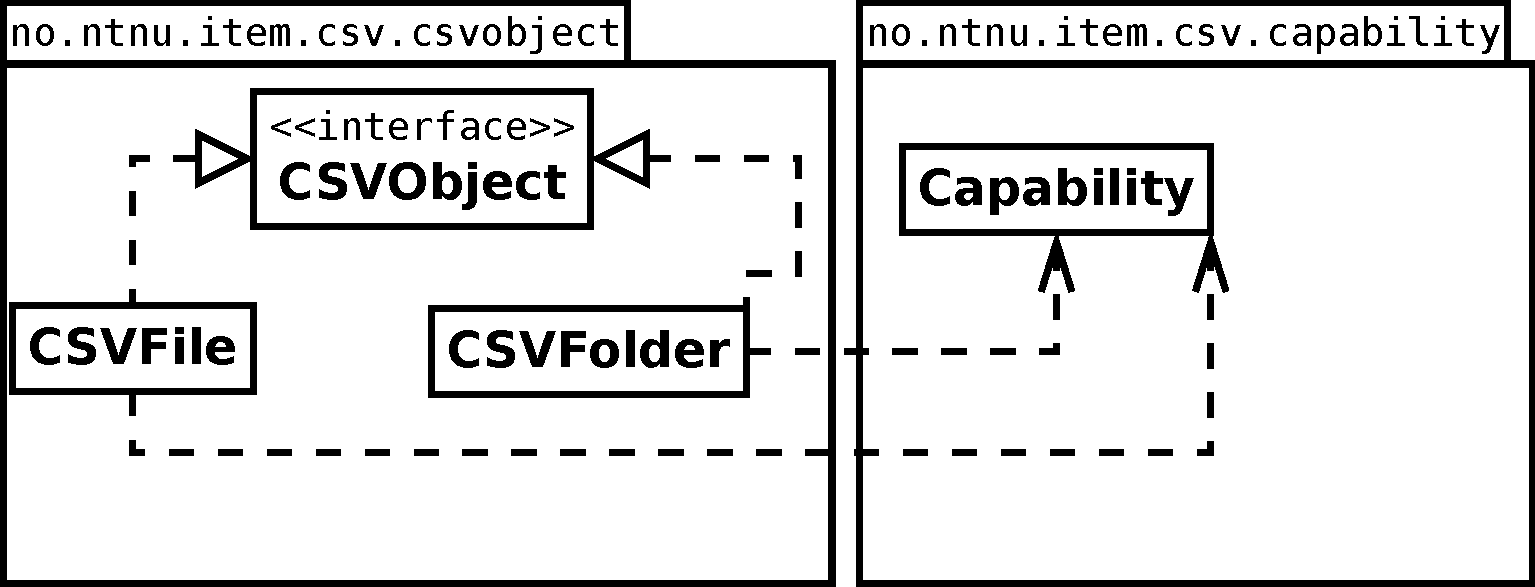
\includegraphics[scale=0.4]{csvobjects.pdf}
    \caption{Cryptographic entities and their relations}
    \label{fig:CSVlib:overview}
\end{figure}

\paragraph{Capabilities} Capabilities are containers for
cryptographic keys and information to identify a corresponding object. A
capability will contain information to identify an object as either a file or a
folder, and have the information to read, write or verify that object.

Capabilities are stored server side in folders, in it's serialized form shown
in Figure \ref{fig:CAP:serial}. \emph{Object Type} specifies if the capability
represents a file or a folder, with values \emph{F} or \emph{D} 
respectively.

\begin{figure}[h!]
    \centering
    
\includegraphics[scale=0.6]{CapabilitySerialization.pdf}
    \caption{Serialized form of a Capability}
    \label{fig:CAP:serial}
\end{figure}

\emph{Key Type} specifies the permissions the key will grant on the object and
can be either \emph{RO} (Read Only), \emph{RW} (Read and write) or \emph{V}
(Verify).

The different parts are separated by the character \textbf{:}. The key and
verify string are encoded in Base32, which means that the 128 bits these
strings are represented by, will be replaced by an alphabet of 32 different
symbols, namely A-Z and 2-7. This transformation will give some overhead in
storage and transfer (26 bytes compared to 16), but makes it possible to read for a human
with few mistakes or misunderstandings.

\paragraph{Folders}

A folder is represented by the class \textbf{CSVFolder}. A CSVFolder object is
a collection of aliases and their corresponding capabilities. For
the most part, the data stored in a folder is so small that it can easily live for 
as long as needed in the memory of the client. 

When a folder is created or updated, the content is serialized and encrypted,
before it is uploaded to the server directly from memory. The serialization for
each item in a folder is simply \textbf{alias;capability}, where the capability
itself is also serialized.

\paragraph{Files}

A file is represented by the class \textbf{CSVFile}. While a folder in general is small,
a file can be of any size, even larger than the space the \ac{RAM} on the
device itself represents. 

To keep the memory footprint low, we use the pipe-and-filter architectural
pattern to stream data all the way from the cloud to the disk, or vice versa,
through encryption and verification. 

An example of how we do this for uploads is shown in Listing
\ref{lst:inputstream}. 

\lstinputlisting[label=lst:inputstream, caption=Pipe and filter upload of a file]
{listings/fileupload_example.java}

The \emph{InputStreams} are chained together, with the effect that a read from
\emph{readBuffer} will trigger a read trough the whole pipe. The
\emph{DigestInputStream} will update the state of the hash function, but is
transparent in the sense that whatever goes into the stream will also be what
comes out. The \emph{CipherInputStream} on the other hand, will output an encrypted
stream of the data from the file. Buffers are placed between each step of the
stream for some performance increase.

\subsubsection{Communication with Server}
% Do not repeat what is said in Server equivalent section
% Apache commons, Serialization of objects

For \ac{HTTP} transport we utilize the Apache Software Foundations
HttpComponents Client\footnote{ \url http://hc.apache.org/} also known as
HttpClient.

This Client offers support for authenticated requests to a server, and both
upload and download through \textbf{PUT} and \textbf{GET} requests respectively.
We wrap communication with the server in two classes,
\texttt{Communication.java} and \texttt{CSVFileManager.java}.
\texttt{Communication.java} provides functionality for sending and retrieving
data from our server, while \texttt{CSVFileManager.java} provides specific
methods for sending and receiving the encrypted objects, CSVFile and CSVFolder.

\subsection{Sharing}
% Sequence Diagram - How we use the cryptographic solutions (and which ones) to
% achieve sharing, securely

A \emph{shared folder} is basically just a folder object which two or more
people have the required encryption keys for. 

The problem of creating a share with someone, is that you have to verify that
you are actually sharing with the correct person. The data, or \emph{secret},
that will have to be shared, is a serialized form of the capability of the
shared folder, as shown in Figure \ref{fig:CAP:serial}.

The client supports two methods of doing this. The most cumbersome
is having to manually copying the key from one users client to another, and
afterwards verifying that the key for the selected folder is correct. An example
of this can be seen in Figure \ref{fig:CSVAndroid:manualimport}. This feature
is also needed to support out-of-band methods for establishing a share. 

\begin{figure}[h!]
    \centering
    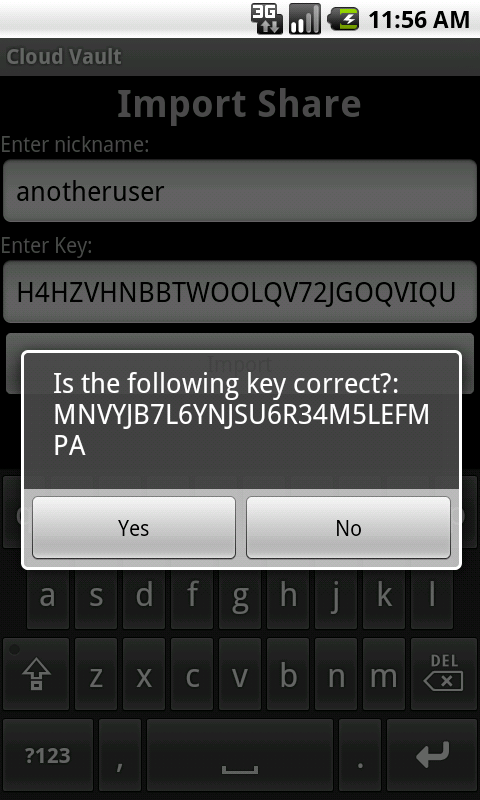
\includegraphics[scale=0.4]{client-manualimport.png}
    \caption{Establishing a share by copying the key}
    \label{fig:CSVAndroid:manualimport}
\end{figure}

The other possibility is to make use of a \ac{QR} code, which is a matrix
barcode that can store information. What this means is that one user will
generate a barcode on his device, and the other user can scan that code using
the camera on his device. Figure \ref{fig:CSVAndroid:barcode} illustrates how
this code will look. The barcode contains both the key and the verification for
the shared folder. Once two users have shared a folder once, that folder can be
used for all future shares, which means that the two people will never have to
meet and do the capability exchange again. The identity has thus been verified.

\begin{figure}[h!]
    \centering
    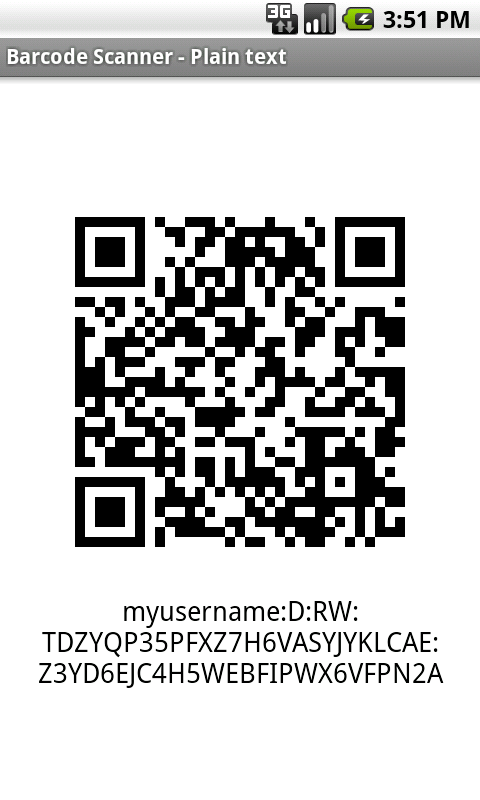
\includegraphics[scale=0.4]{client-barcode.png}
    \caption{Establishing a share by using barcodes}
    \label{fig:csvandroid:barcode}
\end{figure}

\subsection{Adding a new client}

Using more clients, or different devices, is almost the exact same as sharing,
and is solved in the same manner. The only difference is that the capability
that needs to be transfered, is that of the \emph{root folder}. It is also
possible to take any other folder and use as a new root for the new client if
that is the users wish.

\subsection{Securing the client}

For a user to access his root folder, the client will have to know the
capability of that folder. This is clearly to much for a user to remember, so
the capability will have to be stored on the client. However, the client might
be stolen or broken into by some means, and if the capability is stored in clear
text, it is easily stolen. 

We partially remedy this by the use of the \ac{PBKDF2} algorithm, which makes an
encryption key from a password. This generated key is used to encrypt the root
capability in a file stored on the client. We call this the encrypted key ring.

These precautions are however no defense if the attacker managed to read the
memory while the key is unlocked. The client enforces that this password should
be at least 9 characters long. 

\subsection{User Interface}
% goal: As easy as possible!
% First start: Generate new cap/import an old one (Adding a new client section)
% Browsing remote file(s)/folders
% Sharing a file - first/following times - Key Distribution
% Uploading/Downloading file

We have tried to make a user interface that is easily understandable by a novice
user, both in terms of \emph{where to click} and in terms of how we name
cryptographic operations. For instance we never use the word \emph{capability}
in the client.

\paragraph{Main Screen}

The main screen of the application is shown in Figure
\ref{fig:CSVAndroid:mainscreen}. However, before the user gets to this screen,
he will have to unlock his local keyring with his password. If it is the first
time the user starts the application, he will have to enter his online
credentials, and gets a choice to either import an existing root folder, or to
generate a new one. In both cases the user will have to choose a password to
encrypt the root capability in to the local keyring.. From the main screen the
most common action would be to \emph{Browse the vault} -- in other words to see
the files that the user has stored in the cloud.

\begin{figure}[h!]
    \centering
    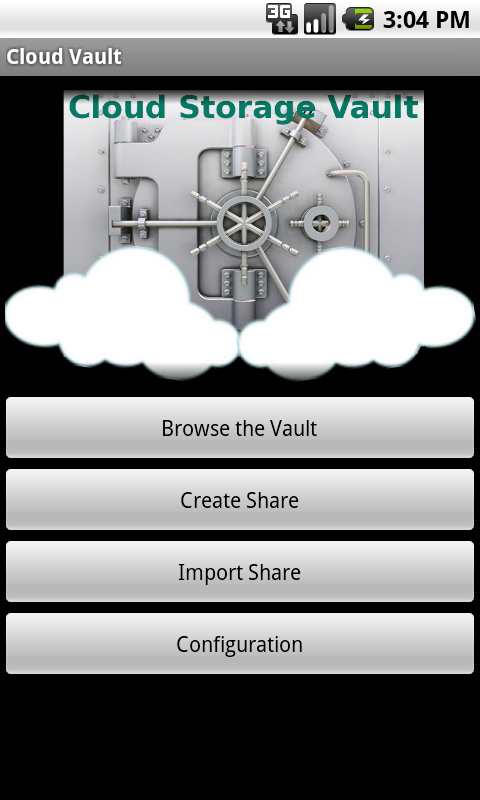
\includegraphics[scale=0.4]{client-mainscreen.png}
    \caption{Main screen of client}
    \label{fig:CSVAndroid:mainscreen}
\end{figure}

\paragraph{Browse the cloud} 

The interface for browsing the files stored in the cloud is made in what we
understand as a common and understandable way of interpreting users actions on
the android platform, and can be seen in Figure
\ref{fig:CSVAndroid:remotebrowse}. Tapping a file will download that file, and
tapping a folder will open that folder. 

\begin{figure}[h!]
    \centering
    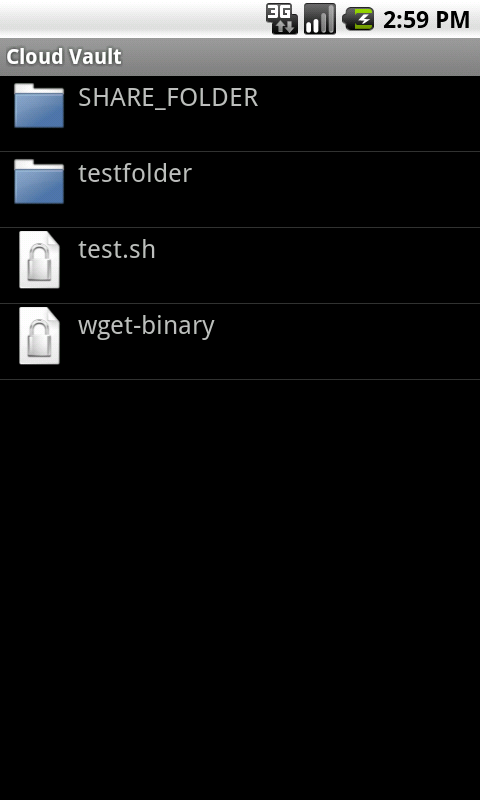
\includegraphics[scale=0.4]{client-remotebrowse.png}
    \caption{Browsing the cloud storage from client}
    \label{fig:CSVAndroid:remotebrowse}
\end{figure}

An upload is treated in a similar way. To reveal this option, the user have to
press the \textbf{Menu}-button. The user will then be allowed to browse his
local filesystem for the file he wishes to upload, and tapping that file will
start the upload. 

A long press on a file, or a folder item, will reveal the context menu shown in
Figure \ref{fig:CSVAndroid:remotecontext}. The least understandable action is
probably \emph{Unlink}, which remove a file or a folder from the parent folder.
The reason why it says unlink and not delete, is that a file can potentially be
linked in a number of different folders, and it is impossible by our design to
reveal which folders the file has been linked to, except the one that we are
unlinking from.

\begin{figure}[h!]
    \centering
    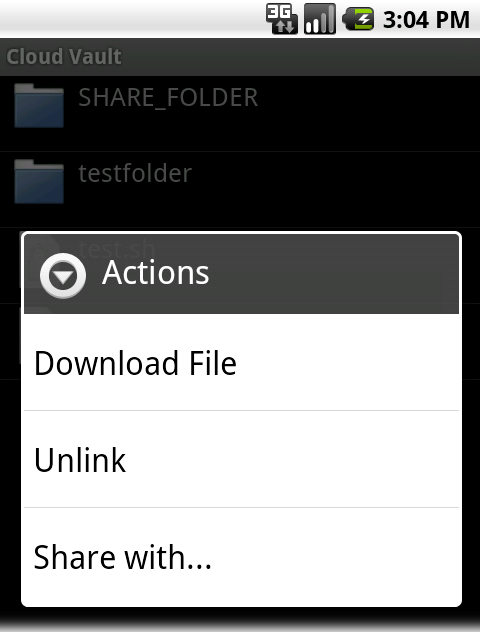
\includegraphics[scale=0.4]{client-browsecontext.png}
    \caption{Context menu}
    \label{fig:CSVAndroid:remotecontext}
\end{figure}

%**************************************%
\chapter{Experimental Procedures}
%**************************************%
This chapter will explain the experimental procedures performed towards the Cloud
Storage Vault. It will start by explaining the
procedures taken to measure the application's performance. The Performance is
further checked against efficiency of similar existing applications.
The chapter will complete by further explaining the experimental procedures
taken to measure the application's security.

\section{Performance}
We have tested the application on two Android phones, a HTC Desire and a HTC
Hero. We have also tested the Java libraries on desktop computer. The
specifications for HTC Desire can be seen in Table \ref{tbl:devices:desire},
for HTC Hero in Table \ref{tbl:devices:hero} and the computer in Table
\ref{table:devices:computer}.

\begin{table}
  \centering
  \caption{HTC Desire Specifications}
  \begin{tabular}{ | l | l |}
    \hline
    Name    & HTC Desire                        \\ \hline
    CPU     & Qualcomm Snapdragon QSD8250, 1 GHz \\ \hline
    Memory  & 576 MB \ac{RAM}                   \\ \hline
    Storage & Samsung Micro SDHC Class 2, 4 GB  \\ \hline
    System  & Android 2.2, Linux 2.6.32.15      \\ \hline
  \end{tabular}
  \label{tbl:device:desire}
\end{table}

\begin{table}
  \centering
  \caption{HTC Hero Specifications}
  \begin{tabular}{ | l | l |}
    \hline
    Name    & HTC Hero                          \\ \hline
    CPU     & Qualcomm MSM7200A, 528 MHz        \\ \hline
    Memory  & 288 MB \ac{RAM}                   \\ \hline
    Storage & Micro SDHC Class 6, 4 GB          \\ \hline
    \ac{OS} & Android 2.2, Linux 2.6.29.6      \\ \hline
  \end{tabular}
  \label{tbl:device:hero}
\end{table}

\begin{table}[!h]
    \centering
    \caption{Test computer Specifications}
    \label{tab:hwbf}
    \begin{tabular}{| l | l |}
	\hline
	Product		        &HP Compaq 8100 Elite SFF PC \\
	\hline
	CPU		            &Intel(R) Core(TM) i7 CPU 860 @ 2.80GHz\\
	\hline
	Memory	            &4GB \ac{RAM}\\
	\hline
    Storage             &Hitachi HDS72105 SATA2 \\
	\hline
    OS		            &Ubuntu 10.10 64 bit\\
	\hline
	Kernel Version	    &Linux 2.6.35\\
	\hline
    Network             &1Gbit wired Ethernet \\
    \hline
    \end{tabular}
\end{table}


\subsection{Eliminating bottlenecks on Android devices}
On the Android devices we identify three possible bottlenecks that we might be
able to control: The Network, our application and the memory card. The mobile
phones will normally obtain their network connection through a wireless
protocol, normally 3G, EDGE or WLAN. While these protocols works just fine,
form a performance standpoint we want to have a fast and stable connection. Our
solution was therefore to connect the Android devices to the test computer, and
use the computers network.

The other bottleneck might be the memory card. The class of a memory will
identify the lowest speed that the card might give on reads. The class number X
represents this guarantee in y MB, so a class 2 card guarantees 2 MB/s. There
are however the possibility of the card performing significantly better than
what the class indicates.

\subsection{What is measured}
% Upload and Download of files (speed/bandwidth). Wget speed, folder creation
% etc
% TODO

\section{Security}

\subsection{Brute Force Local Keyring}
\label{sec:BFLK}
The locally stored and encrypted keyring can be viewed as a weak link, considering lost or hacked user
equipment. Although the keyring is encrypted with a user password, it is still
vulnerable to the old fashion brute force and dictionary attacks. The format of
the encrypted keyring is given in Figure \ref{fig:KeyringFormat}. 

\begin{figure}[h!]
    \centering
    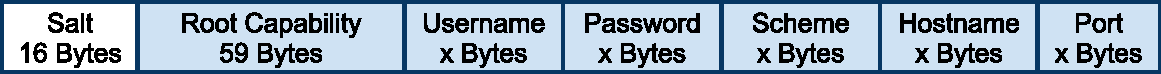
\includegraphics[scale=0.6]{KeyringFormat.pdf}
    \caption{The Keyring format. Encrypted fields are shaded in blue.}
    \label{fig:KeyringFormat}
\end{figure}

\noindent By brute forcing a keyring, a malicious person can retrieve a user's password and server
access data. This will result in a complete failure of security. This section
explains the procedures taken to test the keyring's resistance against brute
force and dictionary attacks. It will start by describing the fundamental procedure for
both attacks, and further explain how the attacks were carried out.

\subsubsection{General Procedure}
The keyring is encrypted with 128-bit AES in ECB mode. The corresponding
encryption key is generated from a user password using PBKDF2 prior to
encryption.\\

\noindent To perform a brute force or dictionary attack against the encrypted
keyring, one must decrypt the keyring for each password guessed. The decryption
involves both key derivation with PBKDF2 and decryption with 128-bit AES in ECB
mode. If a guessed password results in the correct plaintext, it is
considered to be the correct password.In our brute force and dictionary
attacks, we recognized a correct plaintext to contain three ``:'', and with the
first byte set to ``D''.

\subsubsection{Implemented Attacks}
We created two programs designed to crack the keyring password. The first program,
named BruteForce, was designed for a single computer, to test the keyring's
resistance against brute force and dictionary attacks. The second program, named
\ac{CDA} was designed to perform dictionary attacks by a cluster of cooperating
servers. The corresponding source code and .jar file for both programs can be found in the
attached CD-ROM. Implementation details are given in Appendix \ref{ap:RI}.

\subsubsection{Configuration}
To run BruteForce we have to preconfigure the attacking computer. First of
all, the computer is required to have the Java(TM) Cryptography Extension (JCE)
Jurisdiction Policy Files installed with Java. The second and last requirement is that
the computer is configured with \ac{BC} as its primary JCE provider.
A computer will most likely not be able to correctly decryption the encrypted
keyring, without any of these requirements. The policy files and BC provider are
required because the keyring is encrypted using BC version 1.34\footnote{BC version
1.34 is used by default in Android 2.2.}.\\
%TODO: Confirm that BC v.1.34 is default!!!1

\noindent The CDA requires the exact same configuration as the BruteForce
attack, but for each node in the cluster. Another important requirement for CDA
is that the cluster must be configured with Apache Hadoop.\\

\noindent A guide to install Java(TM) Cryptography Extension (JCE) Jurisdiction
Policy Files and a BC provider can be found at \cite{jce+bc}. A simple guide for
running Apache Hadoop in a Multi-Node Cluster using Ubuntu servers can be found
at \cite{cluster}.

\subsubsection{Hardware Specifications}
The hardware specification for the BruteForce attack on a single computer is
given in Table \ref{tab:hwbf}.
\begin{table}[!h]
    \centering
    \caption{Hardware specifications for computer executing the BruteForce
    attack.}
    \label{tab:hwbf}
    \begin{tabular}{| l | l |}
	\hline
	Product		    &HP Compaq 8100 Elite SFF PC \\
	\hline
	CPU		    &Intel(R) Core(TM) i7 CPU 860 @ 2.80GHz\\
	\hline
	CPU Architecture    &x86\_64\\
	\hline
	RAM		    &4GiB\\
	\hline
	OS		    &Ubuntu 10.10 (Maverick Meerkat)\\
	\hline
	Kernel Version	    &2.6.35-28-generic\\
	\hline
    \end{tabular}
\end{table}

\noindent The CDA attack, however, was executed over a cluster of Amazon \ac{EC2}
instances. All instances used were categorized by Amazon as high-CPU extra large
instances. The hardware specification for a single instance, used in the CDA
attack, is given in Table \ref{tab:hwcda}.

    \begin{table}[!h]
    \centering
    \caption{Hardware specifications for cluster instances executing the CDA
    attack.}
    \label{tab:hwcda}
    \begin{tabular}{| l | l |}
	\hline
	Instance Type	    &High-CPU Extra Large Instance\\
	\hline
	CPU		    &Intel(R) Xeon(R) CPU E5410 @ 2.33GHz\\
	\hline
	CPU Architecture    &x86\_64\\
	\hline
	RAM		    &7GiB\\
	\hline
	OS		    &Ubuntu 10.10 (Maverick Meerkat)\\
	\hline
	Kernel Version	    &2.6.35-24-virtual\\
	\hline
	I/O Performance	    &High (as defined by Amazon)\\
	\hline
    \end{tabular}
\end{table}
\subsubsection{Running a Local Brute Force Attack}
The following command was used to execute a brute force
attack:

\lstset{label=lst:bf, caption=Running local brute force attack}
\begin{lstlisting}
$ java -jar BruteForce.jar /path/to/keyring m t
\end{lstlisting}

\noindent In the above command, m is the maximum word length to brute force and t
is the number of threads to use. The ``\$'' sign indicates that the command is
executed by a normal user on a local computer.\\

\noindent As described in Section \ref{sec:PBKDF2}, PBKDF2 can be configured to run a desired
amount of iterations, to slow down/speed up the key derivation. With this
feature, we were able to test the efficiency of brute force attacks against
different amounts of iterations in PBKDF2. Iteration values of 500, 1000, 2000
and 4000 were tested.

\subsubsection{Running a Local Dictionary Attack}
The local dictionary attack was a part of the brute force program above, and was
executed with the following command:

\lstset{label=lst:da, caption=Running local dictionary attack}
\begin{lstlisting}
$ java -jar BruteForce.jar /path/to/keyring /path/to/dictionary t
\end{lstlisting}
\noindent where t equals the number of computing threads to use. The ``\$'' sign
indicates that the command is executed by a normal user on a local computer.\\

\noindent The dictionary attack was also tested against different amounts of iterations in
PBKDF2. Iteration values of 500, 1000, 2000 and 4000 were tested.

\subsubsection{Running a Dictionary Attack in the Cloud}
The CDA attack was carried out over 20 Amazon EC2 high-CPU extra large
instances. One instance was configured as both a Hadoop master and Hadoop slave node, while the
19 remaining instances behaved as slaves. The commands executed
to start the Hadoop master, slaves and their corresponding \ac{HDFS} are shown
in Listing \ref{lst:hadoop}.

\paragraph{Note:}For all upcoming Bash commands, the ``\$'' sign indicates a command
executed from an attackers local computer, while the ``\%'' sign indicates a
remote command executed from the cluster's master node.

\lstset{language=bash, label=lst:hadoop, caption=Starting Hadoop cluster with HDFS}
\begin{lstlisting}
# Logg into the master node
$ ssh -i ec2-key-pair.pem ubuntu@[master_public_hostname]

# Change into Hadoop directory on master node
% cd /path/to/Hadoop/directory

# Start HDFS and initialize master and slave nodes
% bin/start-dfs.sh

# Start a MapReduce cluster from the master node
% bin/start-mapred.sh
\end{lstlisting}
The last command enables the existing
Hadoop cluster to support MapReduce. This is necessary as the CDA
attack is implemented as a map-reduce problem. Details about MapReduce and the
implementation of CDA are given in Appendix \ref{ap:RI}.\\

\noindent When the cluster is correctly up and running, the attacker must
upload the CDA.jar file, a desired dictionary file and the target keyring to the
master node. This can be done using Bash commands such as sftp or scp.\\

\noindent The last requirement, before executing the CDA attack, is to copy the
desired dictionary file and keyring into the HDFS. Copying files from the master
node to the HDFS is done with the following command.

\lstset{language=bash, label=lst:cpHDFS, caption=Copying files into HDFS}
\begin{lstlisting}
% bin/hadoop dfs -put /path/to/file /path/to/file/in/HDFS
\end{lstlisting}

\noindent The CDA attack was further executed on the master node as follows.

\lstset{language=bash, label=lst:CDA, caption=Executing the CDA attack}
\begin{lstlisting}
% bin/hadoop jar /path/to/CDA.jar /HDFSpath/to/dictionary /HDFSpath/to/output/file /HDFSpath/to/keyring s t
\end{lstlisting}
In the above command, ``s'' equals the number of slaves to use in the cluster
and ``t'' equals the number of processing threads to use per slave. In our
experiment we used s=20 and t=8 as there were 20 slaves in the cluster, and each
slave was capable of running 8 threads in parallel.
%**************************************%
\chapter{Results}
%**************************************%
\section{Brute Force Local Keyring}
In Section \ref{sec:BFLK}, we tried to brute force the locally stored keyring,
by implementing and executing two different programs. The first program, named
BruteForce, was designed to run on a single computer, and supports both brute force and
dictionary attacks. The second program, named Cluster Dictionary Attack (CDA), was created to run in a
computational cluster. However, the CDA attack does only support dictionary attacks. The results for
both programs are given below.

\subsection{BruteForce}
With BruteForce we executed both a brute force and a dictionary attack to estimate the
amount of passwords we could brute force within a second. The brute force
and dictionary attacks achieved approximately the same results. However, for
each measurement, the brute force attack turned out to achieve about 50
passwords more per seconds than the dictionary attack. The results for both
attacks are illustrated in Figure \ref{fig:bfres}.

\begin{figure}[!h]
\centering
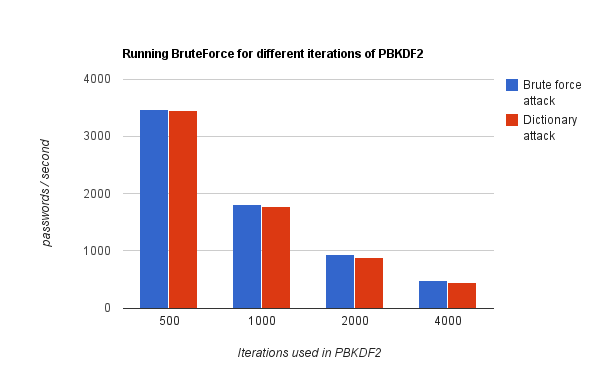
\includegraphics[scale=0.55]{bf.png}
\caption{Results from running brute force and dictionary attacks against a local
keyring. The histogram shows how many passwords per second we were able to brute
force against different amounts of iterations used in PBKDF2.}
\label{fig:bfres}
\end{figure}
\subsection{Cluster Dictionary Attack (CDA)}
In the CDA attack, each node of the cluster achieved approximately the same results as a single computer
running a dictionary attack with BruteForce. With 20 nodes in the cluster we
were able to brute force around 35 000 passwords per second, given PBKDF2 with
1000 iterations.
%**************************************%
\chapter{Discussion}
%**************************************%
\section{Complexity}
% Hvordan vi lagrer filer
% Lagring av nøkler
% Hvordan direktorier fungerer
% Hvordan vi deler

%Vår løsning VS relatert research og existing solutions

\subsection{Keys}

\subsection{Files}

\subsection{Folders}

\subsection{Sharing}

\section{Security}
% Hvordan angripe?
% ACL lag bare ekstra sikkerhet, man kan ikke cracke noe uten keyen!
This thesis is written with the basis that we are hiring storage from an
untrusted provider, and the security of the application should primarily
reflect that. With this starting point we can assume that all data stored on
the server is obtainable by the provider.

\subsection{Passive attacks}
% Avhengig av cryptographic primitives
% Confidentiality den største utfordringen
% Her trengs det gode kilder
The provider will have access to all data on the server, and also know what
data stored is part of files and what is part of folders. The confidentiality
of both files and folders relies primarily on the symmetric cipher used to
encrypt the data. But for folders one can obtain this key if one manages to
obtain the asymmetric private key belonging to the folder. In other words a
folder is attackable both trough the asymmetric and the symmetric cipher used.
If the confidentiality of a folder is breached this will also lead to the
attacker being able to decrypt and subfolders or filer, in contrast the breach
of confidentiality of a file will only compromise that specific file. It is
also important to note that users will use a root folder which any other file
or folder relies on, if the confidentiality of this folder is breached, all
files are effectively compromised.

\subsubsection{Brute Force attacks}
%TODO: Discuss findings with experimental procedure.
\subsubsection{RSA attacks}

\subsubsection{AES attacks}

\subsection{Active attacks}
% MITM - Dersom vi f.eks. skrur av SSL-laget
% Innside attacker - hos Amazon


\subsection{Terminal security}
% What happens if someone steals a terminal
% OR install some backdoor/torjan etc?
Given enough users, at some point there will be a users who looses his
terminal, for instance a mobile phone, a terminal might also be broken into
without the users knowledge.

\section{Performance}
% 1 mappe med 100 filer i, tar ikke mye lenger tid å åpne enn en mappe med 3
% filer i

\section{Omitted features}
% Ting vi ikke har lagt inn
% - Cascading deletes? Loops.
% - Hvem 'eier' en directory
% - Garbage collection? (vanskelig)

\section{Compared with Other Solutions}
%**************************************%
\chapter{Conclusion and Future Work}
%**************************************%

% BibTeX bibliography lives in external file
\bibliographystyle{unsrtnat}
\bibliography{references}
% TODO: Can we fix references in order of apperance?

\appendix
\appendixpage
\addappheadtotoc
% Appendix goes here
\chapter{Relevant Implementations}
\label{ap:RI}
This chapter will study implementation details from applications that were
created, but not a part of the thesis' main topic. Applications considered are 
BruteForce and the Cluster Dictionary Attack (CDA).

\section{BruteForce}
BruteForce includes a plain brute force attack and a dictionary attack against
a users encrypted keyring. Details about the implementation follows.

\subsection{Implementation Details}
BruteForce is written in Java and utilize the javax.crypto library with Bouncy
Castle version 1.34 as JCE provider to decrypt the encrypted keyring. The Bouncy
Castle JCE provider seems to be necessary as Android 2.2 uses it by default to encrypt
the keyring. To enable PBKDF2 before decryption, BruteForce utilize a PBKDF2
Java library available at \cite{pbkdf2}. The program is divided into two
functions named bruteForceAttack and dictionaryAttack that correspondingly executes a brute
force and dictionary attack. The bruteForceAttack function is shown in Listing
\ref{lst:bffunc}.

\lstinputlisting[language=java, label=lst:bffunc, caption=bruteForceAttack
function]{listings/bruteForceAttack.java} 

\noindent bruteForceAttack starts a number of BruteForceThread threads. The
function continues after all BruteForceThreads are initialized and ready to
start their task. It then enters a while-loop. The while-loop executes a pushWord function for each iteration.
The task of pushWord is to simply create and push all possible words of a given length onto
a stack of words. The length of the words to push are given by its integer
argument. The whole attack is based on letting the main thread create and 
push words onto a stack, while the BruteForceThreads are
pulling words from the stack. When a word is pulled from the stack it is
subject to PBKDF2, where the result is used to decrypt the ciphertext. If
decryption results in a given plaintext, the password is found.\\

\noindent The dictionaryAttack function is shown in Listing \ref{lst:dafunc}.

\lstinputlisting[language=java, label=lst:dafunc, caption=dictionaryAttack
function]{listings/dictionaryAttack.java}

dictionaryAttack reads an input dictionary file into a BufferedReader. It then starts
a given number of DictionaryThreads. The DictionaryThreads will read
from the BufferedReader in a synchronized way. When a word is read from a
DictionaryThread it will be subject to PBKDF2, where the result is used to
decrypt the ciphertext. If decryption results in a given
plaintext, the password is found.

\section{Cluster Dictionary Attack}
The CDA is written in Java and is built around the same procedure as the
dictionary attack in BruteForce. However, the difference lays in the cooperation
of multiple computers. To enable a cluster of computers to cooperate, we used
the following environment.

\subsection{Environment}
The environment is based upon a software framework from Apache called Hadoop. The
main functionality of Hadoop is described below.

\subsubsection{Apache Hadoop}
Apache Hadoop makes it possible for multiple machines to cooperate
and run computational work together. Hadoop also provides a distributed filesystem
\ac{HDFS} that can store data across multiple cooperating machines \cite{hadoop}. The
computational work in Hadoop is organized and distributed using MapReduce.
The concept of MapReduce is explained below.

\paragraph{MapReduce} is a programming paradigm introduced by Google. It is designed to
process and generate large sets of data using a cluster of machines \cite{mapred}.
In MapReduce, a large set of input data is divided into multiple key/value
pairs. The key/value pairs are further distributed to multiple MapReduce tasks
running on multiple machines. A MapReduce task is divided into
a mapper and a reducer. The task of a mapper is to perform an operation on a
key/value pair and return a key/value pair as a result to the reducer. The
reducer collects key/value pairs from multiple mappers and combine the results
into one or more output files.

\subsection{Implementation Details} 
The CDA attack is implemented as a MapReduce problem, with a large dictionary
file as the data input set. The dictionary is split into separate
key/value pairs, where each value is a single line in the dictionary and the key
corresponds to the line's offset within the dictionary.\\ 

\noindent The key/value pairs are handled by a map function implemented in CDAMapper. The map function has the
responsibility of checking every word on a single dictionary line. Each line in
the dictionary should contain a certain amount of words. This is to enable the
map function to run multiple threads at the same time, where each thread checks
one or more words. With multiple threads the attack is able to utilize more CPU power
for each running machine in the cluster. A detailed view of the map function is
given in Listing \ref{lst:mapfunc}. 

\lstinputlisting[language=java, label=lst:mapfunc, caption=Mapper function in 
CDAMapper]{listings/mapper.java}

When receiving a key/value pair, the map function first splits the input line
into an array of words called line. It then creates a given number of
DictionaryThread threads and serves each thread a sub array of words from the
line array. Each DictionaryThread will check all of its incoming words similar
to the DictionaryThread in BruteForce. If the correct password is found, the
password will be written to the sysout folder in the machine where the mapper is
running.\\

\noindent A class named Processor initializes the CDA attack by configuring the mapper and
reducer tasks. The number of mappers is set equal to the number of nodes
used in the cluster. This is to ensure that each machine only runs one mapper at
a time. The number of reducers are set to zero, because their behavior in
MapReduce is not needed.


\paragraph{Notice:} The for-loop at line 10 in Listing \ref{lst:mapfunc} requires the number of words
per line, in the dictionary, to be equal to a multiple of the number of threads in use. It is
recommended that the input dictionary follows this requirement. In this
occasion, we have created a Bash script, named dictmaker.sh, that changes a regular dictionary into
an N words-per-line dictionary. The script can be found in the attached CD-ROM.
 
\end{document}
